%-----------------------------------------------------------------------------
%
%               Template for sigplanconf LaTeX Class
%
% Name:         sigplanconf-template.tex
%
% Purpose:      A template for sigplanconf.cls, which is a LaTeX 2e class
%               file for SIGPLAN conference proceedings.
%
% Guide:        Refer to "Author's Guide to the ACM SIGPLAN Class,"
%               sigplanconf-guide.pdf
%
% Author:       Paul C. Anagnostopoulos
%               Windfall Software
%               978 371-2316
%               paul@windfall.com
%
% Created:      15 February 2005
%
%-----------------------------------------------------------------------------


\documentclass{llncs}
\pdfoutput=1

% The following \documentclass options may be useful:
%
% 10pt          To set in 10-point type instead of 9-point.
% 11pt          To set in 11-point type instead of 9-point.
% authoryear    To obtain author/year citation style instead of numeric.

\usepackage{lmodern}
\usepackage[T1]{fontenc}
\usepackage{xspace}
\usepackage{graphicx}
\usepackage{slatex}
\usepackage{subfig}
\usepackage{upgreek}
\usepackage{varwidth}
\usepackage{verbatim}
\usepackage{color}
\usepackage{stmaryrd}
\usepackage{amsmath}
\usepackage{amssymb}
\usepackage{amsthm}
\usepackage{amscd}
\usepackage{mathtools}

\usepackage{xparse}
\makeatletter
\NewDocumentCommand{\raisedminus}{m}{%
  \raisebox{0.2em}{$\m@th#1{-}$}%
}
\NewDocumentCommand{\unaryminus}{}{%
  \mathbin{%
    \mathchoice{%
      \raisedminus\scriptstyle
    }{%
      \raisedminus\scriptstyle
    }{%
      \raisedminus\scriptscriptstyle
    }{%
      \raisedminus\scriptscriptstyle
    }%
  }%
}
\makeatother

% Hyperref likes to go last
\usepackage[
    bookmarks=true,
    bookmarksnumbered=true,
    breaklinks=false,
    raiselinks=true,
    pdfborder={0 0 0},
    colorlinks=false,
    plainpages=false,
    ]{hyperref}

% This makes hyperlinks point to the tops of figures, not their captions
\usepackage[all]{hypcap}

%%%%%%%%%%%%%%%%%%%%%%%%%%%%%%%%%%%%%%%%%%%%%%%%%%%%%%%%%%%%%%%%%%%%%%%%%%%%%%%%%%%%%%%%%%%%%%%%%%%%%
% BEGIN SPACE HACKS
%%%%%%%%%%%%%%%%%%%%%%%%%%%%%%%%%%%%%%%%%%%%%%%%%%%%%%%%%%%%%%%%%%%%%%%%%%%%%%%%%%%%%%%%%%%%%%%%%%%%%

%\usepackage{showframe}

\makeatletter
\renewcommand\normalsize{%
   \@setfontsize\normalsize\@@ptsize{14.5pt}%
   \abovedisplayskip 8\p@ \@plus2\p@ \@minus2\p@
   \belowdisplayskip \abovedisplayskip
   \abovedisplayshortskip 4\p@ \@plus2\p@ \@minus2\p@
   \belowdisplayshortskip \abovedisplayshortskip
   \renewcommand\arraystretch{0.65}
}

\renewcommand\small{%
   \@setfontsize\small\@ixpt{12pt}%
   \abovedisplayskip 7\p@ \@plus2\p@ \@minus2\p@
   \belowdisplayskip \abovedisplayskip
   %\abovedisplayshortskip 0\p@
   %\belowdisplayshortskip 0\p@
   %\belowdisplayskip \abovedisplayskip
   \renewcommand\arraystretch{0.9}
}

%\setlength\floatsep       {3pt \@minus 1\p@}
%\setlength\textfloatsep   {12pt \@minus 4\p@}
%\setlength\intextsep      {3pt \@minus 1\p@}
%\setlength\dblfloatsep    {3pt \@minus 1\p@}
%\setlength\dbltextfloatsep{3pt \@minus 1\p@}
\makeatother

\usepackage{enumitem}
\setlist{noitemsep,topsep=2pt}
\setitemize{noitemsep,topsep=2pt}
\setenumerate{noitemsep,topsep=2pt}

\newcommand{\smallmathfont}{\small}

%%%%%%%%%%%%%%%%%%%%%%%%%%%%%%%%%%%%%%%%%%%%%%%%%%%%%%%%%%%%%%%%%%%%%%%%%%%%%%%%%%%%%%%%%%%%%%%%%%%%%
% END SPACE HACKS
%%%%%%%%%%%%%%%%%%%%%%%%%%%%%%%%%%%%%%%%%%%%%%%%%%%%%%%%%%%%%%%%%%%%%%%%%%%%%%%%%%%%%%%%%%%%%%%%%%%%%

% Hide subsections in TOC
\setcounter{tocdepth}{1}

\newcounter{maththing}\numberwithin{section}{chapter}

\theoremstyle{definition}
\newtheorem{example}{Example}[chapter]

\theoremstyle{plain}
\newtheorem{definition}[example]{Definition}
\newtheorem{theorem}[example]{Theorem}
\newtheorem{lemma}[example]{Lemma}
\newtheorem{corollary}[example]{Corollary}

\newcommand\numberthis{\addtocounter{equation}{1}\tag{\theequation}}

% puts a little space between the \hrule and captions
\belowcaptionskip 0.25\baselineskip
\newcommand{\bottomhrule}{\vspace{3pt}\hrule\vspace{3pt}}

% keywords
\newcommand{\keyword}[1]{\textbf{#1}}
\newcommand{\mykeyword}[1]{\textbf{\textit{#1}}}

\newcommand\xqed[1]{%
  \leavevmode\unskip\penalty9999 \hbox{}\nobreak\hfill
  \quad\hbox{#1}}

\newcommand{\exampleqed}{\xqed{$\diamondsuit$}}


\newcommand{\lzfclang}{\ensuremath{\lambda_{\text{ZFC}}}\xspace}

%
% Language phase 0: meta
%
% Mostly semantic functions and grammars, definitional extensions to first-order logic

\newcommand{\metadef}{:=}
\newcommand{\metastx}{:\equiv}
\newcommand{\objdef}{:=}
\newcommand{\objstx}{:\equiv}
\newcommand{\gor}{\ |\ }
\newcommand{\meaningof}[1]{\left\llbracket{#1}\right\rrbracket}
\newcommand{\enc}[1]{\mathcal{F}\!\meaningof{#1}}
\newcommand{\stx}[1]{\mathcal{S}\!\meaningof{#1}}
%\newcommand{\metasubst}[3]{{#1}[{#2}:={#3}]}
\newcommand{\metasubst}[3]{s\!\meaningof{{#1},{#2},{#3}}}
\newcommand{\imp}{\Rightarrow}
\newcommand{\rimp}{\Leftarrow}
\DeclareMathOperator{\disjoint}{\mbox{$\not\mspace{-5mu}\i$}}

\renewcommand{\dots}{...}
\newcommand{\setb}[2]{\lbrace {#1} \ \lvert\ {#2} \rbrace}

\newcommand{\justdenom}[1]{\mspace{-4mu} {} \atop {#1} \mspace{-4mu}}
\newcommand{\djustdenom}[1]{\displaystyle{\justdenom{#1}}}


%
% Language phase 1: first-order logic
%

% Common notation and names

\newcommand{\set}[1]{\{{#1}\}}
\newcommand{\seq}[1]{\left({#1}\right)}
\newcommand{\pair}[1]{\langle{#1}\rangle}
\newcommand{\dpair}[1]{\left\langle{#1}\right\rangle}

\newcommand{\band}{\wedge}
\newcommand{\pand}{\big\wedge}
\newcommand{\bor}{\vee}
\newcommand{\por}{\big\vee}

\newcommand{\Bool}{\mathbb{B}}
\newcommand{\Nat}{\mathbb{N}}
\newcommand{\Int}{\mathbb{Z}}
\newcommand{\Rat}{\mathbb{Q}}
\renewcommand{\Re}{\mathbb{R}}
\renewcommand{\P}{\mathbb{P}}

\newcommand{\U}{\textstyle\bigcup}
\renewcommand{\u}{\cup}
\newcommand{\I}{\textstyle\bigcap}
\renewcommand{\i}{\cap}
\newcommand{\wo}{\backslash}
\let\oldemptyset\emptyset
\renewcommand{\emptyset}{\varnothing}
\newcommand{\powerset}{\mathcal{P}}

\newcommand{\Forall}[1]{\forall\,{#1}\ldotp\,}
\newcommand{\Exists}[1]{\exists\,{#1}\ldotp\,}
\newcommand{\ExistsOne}[1]{\exists\char`^\,{#1}\ldotp\,}
\newcommand{\The}[1]{\iota\,{#1}\ldotp\,}

\newcommand{\tto}{\Rightarrow}
%\newcommand{\bijto}{\xrightarrow{\mathrm{bij}}}
\newcommand{\bijto}{\leftrightarrow}
\newcommand{\Ord}{\mathit{Ord}}

\newcommand{\A}{\mathcal{A}}
\newcommand{\B}{\mathcal{B}}
\newcommand{\C}{\mathcal{C}}
\newcommand{\E}{\mathcal{E}}
\newcommand{\V}{\mathcal{V}}

\newcommand{\pnand}{\mathit{nand}}
\newcommand{\w}{\backslash}

% Invented notation and names

\newcommand{\myfun}[1]{\mathit{#1}}
\newcommand{\encset}{\myfun{set}}
\newcommand{\lex}{\myfun{lex}}
\newcommand{\addset}{\myfun{put}}

%\newcommand{\dto}{\Downarrow}
% makes the horizontal spacing around the arrow nice:
\DeclareMathOperator{\dto}{\Downarrow}

\newcommand{\plusomega}{+_\lnat}
\newcommand{\timesomega}{\times_\lnat}

\newcommand{\plusint}{+_Z}
\newcommand{\minusint}{-_Z}
\newcommand{\timesint}{\times_Z}
\newcommand{\equalint}{=_{\mathsf{Z}}}

\newcommand{\plusz}{+_\Int}
\newcommand{\minusz}{-_\Int}
\newcommand{\timesz}{\times_\Int}

\newcommand{\equalrat}{=_{\mathsf{Q}}}
\newcommand{\plusq}{+_\Rat}
\newcommand{\minusq}{-_\Rat}
\newcommand{\timesq}{\times_\Rat}
\newcommand{\divq}{\div_\Rat}

%
% Language phase 2: lambda_ZFC
%

\newcommand{\objlang}[1]{\mathsf{#1}}
%\newcommand{\objlang}[1]{\mathtt{#1}}

\renewcommand{\choose}{\mathcal{E}}
%\newcommand{\Choose}[1]{\choose\,{#1}\ldotp\,}
\newcommand{\Choose}[1]{\set{#1}\ldotp\,}

\newcommand{\domain}{\objlang{domain}}
\newcommand{\range}{\objlang{range}}
\newcommand{\image}{\objlang{image}}
\newcommand{\filter}{\objlang{select}}

\newcommand{\lunion}[1]{{\textstyle\U}\ {#1}}
\newcommand{\lpowerset}[1]{\powerset\ {#1}}
\newcommand{\limage}[2]{{\objlang{image}}\ {#1}\ {#2}}
\newcommand{\lorder}[1]{{\objlang{card}}\ {#1}}
\newcommand{\ltake}[1]{{\objlang{take}}\ {#1}}
\newcommand{\lemptyset}{\oldemptyset}
\newcommand{\lnat}{\upomega}
\newcommand{\lif}[3]{{\objlang{if}}\ {#1}\ {#2}\ {#3}}
\newcommand{\ltrue}{\objlang{true}}
\newcommand{\lfalse}{\objlang{false}}
\newcommand{\lfun}{\lambda\ldotp\,}

\newcommand{\fun}[1]{\lambda\mspace{2mu}{#1}\ldotp\,}

\newcommand{\tvar}{t_\mathrm{var}}
\newcommand{\tapp}{t_\mathrm{app}}
\newcommand{\tif}{t_\mathrm{if}}
\newcommand{\tin}{t_\in}
\newcommand{\tunion}{t_\u}
\newcommand{\ttake}{t_\mathrm{take}}
\newcommand{\tpowerset}{t_\powerset}
\newcommand{\timage}{t_\mathrm{image}}
\newcommand{\torder}{t_\mathrm{card}}
\newcommand{\tset}{t_\mathrm{set}}
\newcommand{\tatom}{t_\mathrm{atom}}
\newcommand{\tfun}{t_\lambda}
\newcommand{\atrue}{a_\mathrm{true}}
\newcommand{\afalse}{a_\mathrm{false}}
\newcommand{\ttrue}{t_\mathrm{true}}
\newcommand{\tfalse}{t_\mathrm{false}}

\newcommand{\Vatom}{V_\mathrm{atom}}
\newcommand{\Vset}{V_\mathrm{set}}
\newcommand{\Vfun}{V_\lambda}
\newcommand{\Evar}{E_\mathrm{var}}
\newcommand{\Eapp}{E_\mathrm{app}}
\newcommand{\Eset}{E_\mathrm{set}}
\newcommand{\Eif}{E_\mathrm{if}}
\newcommand{\Ein}{E_\in}
\newcommand{\Eunion}{E_\u}
\newcommand{\Epowerset}{E_\powerset}
\newcommand{\Eimage}{E_\mathrm{image}}
\newcommand{\Eorder}{E_\mathrm{card}}

\newcommand{\fst}{\myfun{fst}}
\newcommand{\snd}{\myfun{snd}}

\newcommand{\jand}{\;\;\,}

\newenvironment{displaybreaks}%
{%
	\begingroup%
	\allowdisplaybreaks%
}%
{%
	\endgroup%
	\ignorespacesafterend%
}

%\excludecomment{proof}

\newcommand{\figref}[1]{Fig.~\ref{#1}}
\newcommand{\figsref}[1]{Figs.~\ref{#1}}

\newcommand{\arrow}{\rightsquigarrow}

\newcommand{\restrict}[1]{\lvert_{#1}}
\newcommand{\pto}{\rightharpoonup}
\newcommand{\Un}{\mathcal{U}}

\newcommand{\join}{\vee}

\newcommand{\conv}{^{\mspace{-2mu}\Downarrow\mspace{-2mu}}}

\newcommand{\meaningofconv}[1]{\left\llbracket{#1}\right\rrbracket\conv}

\newcommand{\arrowlift}{\ensuremath{lift}}
\newcommand{\arrowarr}{\ensuremath{arr}}
\newcommand{\arrowcomp}{\ensuremath{{>}\mspace{-6mu}{>}\mspace{-6mu}{>}}}
\newcommand{\arrowpair}{\ensuremath{\mathit{\&\mspace{-7.5mu}\&\mspace{-7.5mu}\&}}}
\newcommand{\arrowif}{\ensuremath{ifte}}
\newcommand{\arrowconvif}{\ensuremath{ifte\conv}}
\newcommand{\arrowlazy}{\ensuremath{lazy}}
\newcommand{\arrowapp}{\ensuremath{app}}
\newcommand{\arrowrun}{\ensuremath{run}}
\newcommand{\arrowget}{\ensuremath{get}}
\newcommand{\arrowerror}{\ensuremath{error}}
\newcommand{\arrowtrans}{\ensuremath{\eta}}

\newcommand{\gen}{_\mathrm{a}}
\newcommand{\genb}{_\mathrm{b}}
\newcommand{\genc}{_\mathrm{a^{\mspace{-2mu}*}}}
\newcommand{\gend}{_\mathrm{b^{\mspace{-2mu}*}}}

\DeclareMathOperator{\botto}{\arrow_{\mspace{-3mu}\bot}}
\newcommand{\arrbot}{\arrowarr_{\mspace{-3mu}\bot}}
\newcommand{\compbot}{\arrowcomp_{\mspace{-5mu}\bot}}
\newcommand{\pairbot}{\arrowpair_{\mspace{-3mu}\bot}}
\newcommand{\ifbot}{\arrowif_{\mspace{-2mu}\bot}}
\newcommand{\lazybot}{\arrowlazy_{\mspace{-2mu}\bot}}

\newcommand{\map}{_\mathrm{map}}
\DeclareMathOperator{\mapto}{\arrow_{\mspace{-21mu}\map}}
\newcommand{\liftmap}{\arrowlift\map}
\newcommand{\arrmap}{\arrowarr\map}
\newcommand{\compmap}{\arrowcomp\map}
\newcommand{\pairmap}{\arrowpair\map}
\newcommand{\ifmap}{\arrowif\map}
\newcommand{\lazymap}{\arrowlazy\map}

\newcommand{\pre}{_\mathrm{pre}}
\DeclareMathOperator{\preto}{\arrow_{\mspace{-19mu}\pre}}
\newcommand{\liftpre}{\arrowlift\pre}
\newcommand{\arrpre}{\arrowarr\pre}
\newcommand{\comppre}{\arrowcomp\pre}
\newcommand{\pairpre}{\arrowpair\pre}
\newcommand{\ifpre}{\arrowif\pre}
\newcommand{\lazypre}{\arrowlazy\pre}

\newcommand{\pbot}{{\bot^{\mspace{-4mu}*}}}
\DeclareMathOperator{\pbotto}{\arrow_{\mspace{-3mu}\pbot}}
\newcommand{\arrpbot}{\arrowarr_{\mspace{-3mu}\pbot}}
\newcommand{\comppbot}{\arrowcomp_{\mspace{-5mu}\pbot}}
\newcommand{\pairpbot}{\arrowpair_{\mspace{-3mu}\pbot}}
\newcommand{\ifpbot}{\arrowif_{\mspace{-2mu}\pbot}}
\newcommand{\convifpbot}{\arrowconvif_{\mspace{-2mu}\pbot}}
\newcommand{\lazypbot}{\arrowlazy_{\mspace{-2mu}\pbot}}

\newcommand{\pmap}{_\mathrm{map^{\mspace{-2mu}*}}}
\DeclareMathOperator{\pmapto}{\arrow_{\mspace{-22mu}_{\mathrm{map*}}}}
\newcommand{\liftpmap}{\arrowlift\pmap}
\newcommand{\arrpmap}{\arrowarr\pmap}
\newcommand{\comppmap}{\arrowcomp\pmap}
\newcommand{\pairpmap}{\arrowpair\pmap}
\newcommand{\ifpmap}{\arrowif\pmap}
\newcommand{\convifpmap}{\arrowconvif\pmap}
\newcommand{\lazypmap}{\arrowlazy\pmap}

\newcommand{\ppre}{_\mathrm{pre^{\mspace{-2mu}*}}}
\DeclareMathOperator{\ppreto}{\arrow_{\mspace{-19mu}_{\mathrm{pre*}}}}
\newcommand{\liftppre}{\arrowlift\ppre}
\newcommand{\arrppre}{\arrowarr\ppre}
\newcommand{\compppre}{\arrowcomp\ppre}
\newcommand{\pairppre}{\arrowpair\ppre}
\newcommand{\ifppre}{\arrowif\ppre}
\newcommand{\convifppre}{\arrowconvif\ppre}
\newcommand{\lazyppre}{\arrowlazy\ppre}

\newcommand{\prepto}{\pto_{\mspace{-19mu}\pre}}

\DeclareMathVersion{sans}
\SetSymbolFont{operators}{sans}{T1}{\sfdefault}{m}{n}
\SetSymbolFont{letters}{sans}{T1}{\sfdefault}{m}{n}
\SetMathAlphabet\mathbf{sans}{T1}{\sfdefault}{bx}{n}
\SetMathAlphabet\mathsf{sans}{T1}{\sfdefault}{m}{n}
\SetMathAlphabet\mathit{sans}{T1}{\rmdefault}{m}{it}

\DeclareSymbolFont{greekletters}{OML}{cmss}{m}{n}
\DeclareMathSymbol{\Gamma}  {\mathord}{greekletters}{"00}
\DeclareMathSymbol{\Delta}  {\mathord}{greekletters}{"01}
\DeclareMathSymbol{\Theta}  {\mathord}{greekletters}{"02}
\DeclareMathSymbol{\Lambda} {\mathord}{greekletters}{"03}
\DeclareMathSymbol{\Xi}     {\mathord}{greekletters}{"04}
\DeclareMathSymbol{\Pi}     {\mathord}{greekletters}{"05}
\DeclareMathSymbol{\Sigma}  {\mathord}{greekletters}{"06}
\DeclareMathSymbol{\Upsilon}{\mathord}{greekletters}{"07}
\DeclareMathSymbol{\Phi}    {\mathord}{greekletters}{"08}
\DeclareMathSymbol{\Psi}    {\mathord}{greekletters}{"09}
\DeclareMathSymbol{\Omega}  {\mathord}{greekletters}{"0A}

\DeclareMathSymbol{\alpha}{\mathord}{greekletters}{"0B}
\DeclareMathSymbol{\beta}{\mathord}{greekletters}{"0C}
\DeclareMathSymbol{\gamma}{\mathord}{greekletters}{"0D}
\DeclareMathSymbol{\delta}{\mathord}{greekletters}{"0E}
\DeclareMathSymbol{\epsilon}{\mathord}{greekletters}{"0F}
\DeclareMathSymbol{\zeta}{\mathord}{greekletters}{"10}
\DeclareMathSymbol{\eta}{\mathord}{greekletters}{"11}
\DeclareMathSymbol{\theta}{\mathord}{greekletters}{"12}
\DeclareMathSymbol{\iota}{\mathord}{greekletters}{"13}
\DeclareMathSymbol{\kappa}{\mathord}{greekletters}{"14}
\DeclareMathSymbol{\lambda}{\mathord}{greekletters}{"15}
\DeclareMathSymbol{\mu}{\mathord}{greekletters}{"16}
\DeclareMathSymbol{\nu}{\mathord}{greekletters}{"17}
\DeclareMathSymbol{\xi}{\mathord}{greekletters}{"18}
\DeclareMathSymbol{\pi}{\mathord}{greekletters}{"19}
\DeclareMathSymbol{\rho}{\mathord}{greekletters}{"1A}
\DeclareMathSymbol{\sigma}{\mathord}{greekletters}{"1B}
\DeclareMathSymbol{\tau}{\mathord}{greekletters}{"1C}
\DeclareMathSymbol{\upsilon}{\mathord}{greekletters}{"1D}
\DeclareMathSymbol{\phi}{\mathord}{greekletters}{"1E}
\DeclareMathSymbol{\chi}{\mathord}{greekletters}{"1F}
\DeclareMathSymbol{\psi}{\mathord}{greekletters}{"20}
\DeclareMathSymbol{\omega}{\mathord}{greekletters}{"21}
\DeclareMathSymbol{\varepsilon}{\mathord}{greekletters}{"22}
\DeclareMathSymbol{\vartheta}{\mathord}{greekletters}{"23}
\DeclareMathSymbol{\varpi}{\mathord}{greekletters}{"24}
\DeclareMathSymbol{\varrho}{\mathord}{greekletters}{"25}
\DeclareMathSymbol{\varsigma}{\mathord}{greekletters}{"26}

\DeclareSymbolFont{fixpunct}{T1}{\rmdefault}{m}{n}
\DeclareSymbolFont{fixpunctoml}{OML}{\rmdefault}{m}{n}
\DeclareMathSymbol{,}{\mathpunct}{fixpunct}{`,}
\DeclareMathSymbol{.}{\mathord}{fixpunct}{`.}
\DeclareMathSymbol{\ldotp}{\mathord}{fixpunct}{`.}
\DeclareMathSymbol{!}{\mathord}{letters}{`-}
\DeclareMathSymbol{/}{\mathpunct}{fixpunct}{`/}
\DeclareMathSymbol{\rightharpoonup}{\mathrel}{fixpunctoml}{"2A}
\DeclareMathSymbol{^}{\mathpunct}{fixpunct}{`!}

\DeclareSymbolFont{numbers}{T1}{pvh}{m}{n}
\SetSymbolFont{numbers}{sans}{T1}{\rmdefault}{m}{n}
\DeclareMathSymbol{0}{\mathalpha}{numbers}{"30}
\DeclareMathSymbol{1}{\mathalpha}{numbers}{"31}
\DeclareMathSymbol{2}{\mathalpha}{numbers}{"32}
\DeclareMathSymbol{3}{\mathalpha}{numbers}{"33}
\DeclareMathSymbol{4}{\mathalpha}{numbers}{"34}
\DeclareMathSymbol{5}{\mathalpha}{numbers}{"35}
\DeclareMathSymbol{6}{\mathalpha}{numbers}{"36}
\DeclareMathSymbol{7}{\mathalpha}{numbers}{"37}
\DeclareMathSymbol{8}{\mathalpha}{numbers}{"38}
\DeclareMathSymbol{9}{\mathalpha}{numbers}{"39}

\renewcommand{\notin}{\not\in}

\newcommand\mathtest[2]{\mathchoice{#1}{#2}{#2}{#2}}

\newenvironment{lzfcenv}[1][l]%
{%
	\begin{array}[t]{@{}#1@{}}%
}%
{%
	\end{array}%
}

\newcommand{\tab}{\ \ \ }

\newcommand{\lzfc}[2][l]{\begin{lzfcenv}[#1]#2\end{lzfcenv}}
\newcommand{\tlzfc}[1]{\ensuremath{#1}}

\newcommand{\lzfcsplit}[2][@{}]{\lzfc[r #1 l]{#2}}

\newcommand{\lzfclet}[2]{\lzfc{let\ \ \lzfc[r@{\ \objdef\ }l]{#1} \\ \lzfc{\tab in\ \ #2}}}
\newcommand{\lzfccond}[2][\ \longrightarrow\ ]{\lzfc{cond\ \ \lzfc[l@{\ {#1}\ }l]{#2}}}
\newcommand{\lzfccase}[3][\ \longrightarrow\ ]{\lzfc{case\ \ {#2}\\\ \ \lzfc[l@{\ {#1}\ }l]{#3}}}

\newcommand{\dash}{\text{-}}

%
% Racket syntax (must be last - or at least \defschememathescape must be - see last line)
%

% DrRacket's default colors
\definecolor{identifiercolor}{rgb}{0.15,0.15,0.5}
\definecolor{keywordcolor}{rgb}{0.0,0.0,0.0}
\definecolor{constantcolor}{rgb}{0.16,0.5,0.15}
\definecolor{parenthesiscolor}{rgb}{0.52,0.24,0.14}

\def\keywordfont#1{\textcolor{keywordcolor}{#1}}
\def\variablefont#1{\textcolor{identifiercolor}{#1}}
\def\constantfont#1{\textcolor{constantcolor}{#1}}
\def\datafont#1{\textcolor{parenthesiscolor}{#1}}

\makeatletter
\def\mycodehook{\tt\color{parenthesiscolor}\@setfontsize\small{10pt}{11pt minus0.5pt}}
\makeatother
\let\schemecodehook\mycodehook
\setlength{\leftcodeskip}{\parindent}

\setlength{\leftcodeskip}{0pt}
\setlength{\rightcodeskip}{0pt plus 1fil}
\setlength{\abovecodeskip}{0.5\abovedisplayskip}
\setlength{\belowcodeskip}{0.5\belowdisplayskip}

\unsetspecialsymbol{.}
\unsetspecialsymbol{...}
\unsetspecialsymbol{-}
\unsetspecialsymbol{1-}
\unsetspecialsymbol{-1+}

\setspecialsymbol{<blank-line>}{\va{}}
\setspecialsymbol{lambda}{\va{$\mathtt{\lambda}$}}
\setspecialsymbol{λ}{\va{$\mathtt{\lambda}$}}
\setspecialsymbol{~}{\va{$\mathtt{\sim}$}}
\setspecialsymbol{_}{\va{$\underbar{ }$}}
\setspecialsymbol{Omega}{\va{$\mathtt{\Omega}$}}
\setspecialsymbol{omega}{\va{$\mathtt{\omega}$}}
\setspecialsymbol{Ω}{\va{$\mathtt{\Omega}$}}
\setspecialsymbol{ω}{\va{$\mathtt{\omega}$}}

\setkeyword{define/drbayes struct/drbayes}

\defschememathescape{$}


\newsavebox{\codebox}

\renewcommand{\paragraph}[1]{\vspace{0.5\baselineskip}\noindent\textbf{{#1}.}\hspace{0.25\baselineskip}}
\newcommand{\smallmathfont}{\fontsize{7.5}{9}\selectfont}

%\newcommand{\todo}[1]{[XXX: {#1}]}
\newcommand{\todo}[1]{}

\newenvironment{displaybreaks}%
{%
	\begingroup%
	\allowdisplaybreaks%
}%
{%
	\endgroup%
	\ignorespacesafterend%
}

\excludecomment{proof}

\newcommand{\figref}[1]{Fig.~\ref{#1}}
\newcommand{\figsref}[1]{Figs.~\ref{#1}}

\newcommand{\arrow}{\rightsquigarrow}

\newcommand{\restrict}[1]{\lvert_{#1}}
\newcommand{\pto}{\rightharpoonup}
\newcommand{\Univ}{\mathbb{U}}
\newcommand{\Un}{\mathcal{U}}

\newcommand{\join}{\vee}

\newcommand{\conv}{^{\mspace{-2mu}\Downarrow\mspace{-2mu}}}

\newcommand{\meaningofconv}[1]{\left\llbracket{#1}\right\rrbracket\conv}

\newcommand{\arrowlift}{\ensuremath{lift}}
\newcommand{\arrowarr}{\ensuremath{arr}}
\newcommand{\arrowcomp}{\ensuremath{{>}\mspace{-6mu}{>}\mspace{-6mu}{>}}}
\newcommand{\arrowpair}{\ensuremath{\mathit{\&\mspace{-7.5mu}\&\mspace{-7.5mu}\&}}}
\newcommand{\arrowif}{\ensuremath{ifte}}
\newcommand{\arrowconvif}{\ensuremath{ifte\conv}}
\newcommand{\arrowlazy}{\ensuremath{lazy}}
\newcommand{\arrowapp}{\ensuremath{app}}
\newcommand{\arrowrun}{\ensuremath{run}}
\newcommand{\arrowget}{\ensuremath{get}}
\newcommand{\arrowerror}{\ensuremath{error}}
\newcommand{\arrowtrans}{\ensuremath{\eta}}

\newcommand{\gen}{_\mathrm{a}}
\newcommand{\genb}{_\mathrm{b}}
\newcommand{\genc}{_\mathrm{a^{\mspace{-2mu}*}}}
\newcommand{\gend}{_\mathrm{b^{\mspace{-2mu}*}}}

\DeclareMathOperator{\botto}{\arrow_{\mspace{-3mu}\bot}}
\newcommand{\arrbot}{\arrowarr_{\mspace{-3mu}\bot}}
\newcommand{\compbot}{\arrowcomp_{\mspace{-5mu}\bot}}
\newcommand{\pairbot}{\arrowpair_{\mspace{-3mu}\bot}}
\newcommand{\ifbot}{\arrowif_{\mspace{-2mu}\bot}}
\newcommand{\lazybot}{\arrowlazy_{\mspace{-2mu}\bot}}

\newcommand{\map}{_\mathrm{map}}
\DeclareMathOperator{\mapto}{\arrow_{\mspace{-21mu}\map}}
\newcommand{\liftmap}{\arrowlift\map}
\newcommand{\arrmap}{\arrowarr\map}
\newcommand{\compmap}{\arrowcomp\map}
\newcommand{\pairmap}{\arrowpair\map}
\newcommand{\ifmap}{\arrowif\map}
\newcommand{\lazymap}{\arrowlazy\map}

\newcommand{\pre}{_\mathrm{pre}}
\DeclareMathOperator{\preto}{\arrow_{\mspace{-19mu}\pre}}
\newcommand{\liftpre}{\arrowlift\pre}
\newcommand{\arrpre}{\arrowarr\pre}
\newcommand{\comppre}{\arrowcomp\pre}
\newcommand{\pairpre}{\arrowpair\pre}
\newcommand{\ifpre}{\arrowif\pre}
\newcommand{\lazypre}{\arrowlazy\pre}

\newcommand{\pbot}{{\bot^{\mspace{-4mu}*}}}
\DeclareMathOperator{\pbotto}{\arrow_{\mspace{-3mu}\pbot}}
\newcommand{\arrpbot}{\arrowarr_{\mspace{-3mu}\pbot}}
\newcommand{\comppbot}{\arrowcomp_{\mspace{-5mu}\pbot}}
\newcommand{\pairpbot}{\arrowpair_{\mspace{-3mu}\pbot}}
\newcommand{\ifpbot}{\arrowif_{\mspace{-2mu}\pbot}}
\newcommand{\convifpbot}{\arrowconvif_{\mspace{-2mu}\pbot}}
\newcommand{\lazypbot}{\arrowlazy_{\mspace{-2mu}\pbot}}

\newcommand{\pmap}{_\mathrm{map^{\mspace{-2mu}*}}}
\DeclareMathOperator{\pmapto}{\arrow_{\mspace{-22mu}_{\mathrm{map*}}}}
\newcommand{\liftpmap}{\arrowlift\pmap}
\newcommand{\arrpmap}{\arrowarr\pmap}
\newcommand{\comppmap}{\arrowcomp\pmap}
\newcommand{\pairpmap}{\arrowpair\pmap}
\newcommand{\ifpmap}{\arrowif\pmap}
\newcommand{\convifpmap}{\arrowconvif\pmap}
\newcommand{\lazypmap}{\arrowlazy\pmap}

\newcommand{\ppre}{_\mathrm{pre^{\mspace{-2mu}*}}}
\DeclareMathOperator{\ppreto}{\arrow_{\mspace{-19mu}_{\mathrm{pre*}}}}
\newcommand{\liftppre}{\arrowlift\ppre}
\newcommand{\arrppre}{\arrowarr\ppre}
\newcommand{\compppre}{\arrowcomp\ppre}
\newcommand{\pairppre}{\arrowpair\ppre}
\newcommand{\ifppre}{\arrowif\ppre}
\newcommand{\convifppre}{\arrowconvif\ppre}
\newcommand{\lazyppre}{\arrowlazy\ppre}

\newcommand{\prepto}{\pto_{\mspace{-19mu}\pre}}

\title{Running Probabilistic Programs Backwards}

\author{\tab\tab Neil Toronto$^1$ \tab\tab\tab\tab\tab Jay McCarthy$^2$ \tab\tab\tab David Van Horn$^1$ \\
\footnotesize{\texttt{neil.toronto@gmail.com} \tab \texttt{jay.mccarthy@gmail.com} \tab \texttt{dvanhorn@cs.umd.edu}}}
\institute{$^1$University of Maryland, College Park \tab $^2$Vassar College}

\date{}

\begin{document}

\maketitle

\begin{abstract}
Many probabilistic programming languages allow programs to be run under constraints in order to carry out Bayesian inference.
Running programs under constraints \emph{could} enable other uses such as rare event simulation and probabilistic verification---except that all such probabilistic languages are necessarily limited because they are defined or implemented in terms of an impoverished theory of probability.
Measure-theoretic probability provides a more general foundation, but its generality makes finding computational content difficult.

We develop a measure-theoretic semantics for a first-order probabilistic language with recursion, which interprets programs as functions that compute preimages.
Preimage functions are generally uncomputable, so we derive an approximating semantics.
We implement the approximating semantics and use the implementation to carry out Bayesian inference, stochastic ray tracing (a rare event simulation), and probabilistic verification of floating-point error bounds.
\end{abstract}

\keywords Probability, Semantics, Domain-Specific Languages

%%%%%%%%%%%%%%%%%%%%%%%%%%%%%%%%%%%%%%%%%%%%%%%%%%%%%%%%%%%%%%%%%%%%%%%%%%%%%%%%%%%%%%%%%%%%%%%%%%%%%
%%%%%%%%%%%%%%%%%%%%%%%%%%%%%%%%%%%%%%%%%%%%%%%%%%%%%%%%%%%%%%%%%%%%%%%%%%%%%%%%%%%%%%%%%%%%%%%%%%%%%
%%%%%%%%%%%%%%%%%%%%%%%%%%%%%%%%%%%%%%%%%%%%%%%%%%%%%%%%%%%%%%%%%%%%%%%%%%%%%%%%%%%%%%%%%%%%%%%%%%%%%

\mathversion{sans}

\section{Introduction}

One key feature usually distinguishes a probabilistic programming language from general-purpose languages: finding the probabilistic conditions under which stated constraints are satisfied.
Often, a probabilistic program simulates a real-world random process and the constraints represent observed, real-world outcomes.
Running the program under the constraints \emph{infers causes from effects}.

Inferring probabilistic causes from observed outcomes is called \keyword{Bayesian inference}, a technique used widely in artificial intelligence.
It has been successful in analyzing phenomena at all scales, from genomes to celestial bodies.
Automating it is one of the primary drivers of probabilistic language development.

One of the simplest probabilistic programs that allows us to demonstrate Bayesian inference simulates the following process of flipping two coins.
\begin{enumerate}
	\item Flip a fair coin; call the outcome $x$.
	\item If $x$ is heads, flip another fair coin. If $x$ is tails, flip an unfair coin with heads probability $0.3$ (tails probability $0.7$). In either case, call the outcome $y$.
\end{enumerate}
The following probabilistic program simulates this process.
\begin{equation}
	\lzfclet{
		x & flip~0.5 \\
		y & flip~(if~(x = heads)~0.5~0.3)
	}{\pair{x,y}}
\label{eqn:coins-program}
\end{equation}
Here, $flip~q$ returns $heads$ with probability $q$ and $tails$ with probability $1-q$.

The meaning of~\eqref{eqn:coins-program} is not the returned random value, but a \keyword{probability distribution} that describes the likelihoods of all possible returned random values.
For discrete processes, this distribution can always be defined by a \keyword{probability mass function}: a mapping from possible values to their probabilities.
These probabilities are computed by multiplying the probabilities of intermediate random values.
For example, the probability of $\pair{heads,heads}$ is $0.5 \cdot 0.5 = 0.25$, and the probability of $\pair{tails,heads}$ (i.e. the second flip is unfair) is $0.5 \cdot 0.3 = 0.15$.
The meaning of~\eqref{eqn:coins-program} is thus the probability mass function
\begin{equation}
	p\ :=\ \big[
		\lzfcsplit{\pair{heads,heads} \mapsto 0.25,\, &\pair{heads,tails} \mapsto 0.25, \\
			\pair{tails,heads} \mapsto 0.15,\, &\pair{tails,tails} \mapsto 0.35 \big]}
\end{equation}
Using $p$, we can answer any question about the process under constraints.
For example, if we do not know $x$, but constrain $y$ to be $heads$, what is the probability that $x$ is also $heads$?
We compute the answer by dividing the probability of the outcome we are interested in ($x$ and $y$ are both $heads$) by the total probability of outcomes in the constraint's corresponding subdomain $\set{heads,tails} \times \set{heads}$:
\begin{equation}
	\frac{p~\pair{heads,heads}}{\sum_{z \in \set{heads,tails} \times \set{heads}} p~z} \ =\ 
	%\frac{p~\pair{heads,heads}}{p~\pair{heads,heads} + p~\pair{tails,heads}} \ =\ 
	\frac{0.25}{0.25 + 0.15}\ =\ 0.625
\label{eqn:prob-heads-heads}
\end{equation}
Qualitatively, $y$ being $heads$ is a bit unusual if the second coin is unfair.
Therefore, we infer that the second coin is most probably fair; i.e. $x$ is most likely $heads$.

The time complexity of computing $p$ is generally exponential in the number of random choices, which is intractable for all but the simplest processes.
One popular way to avoid this exponential explosion is to use advanced Monte Carlo algorithms to sample according to $p$ on the constraint's corresponding subdomain without explicitly enumerating that subdomain.
The number of required samples is typically quadratic in the answer's desired accuracy.

\begin{figure*}[!tb]\centering
%\smallmathfont%
\subfloat[Simulated photons from a single source, constrained to pass through an aperture.]{
\begin{minipage}{0.49\textwidth}
\centering
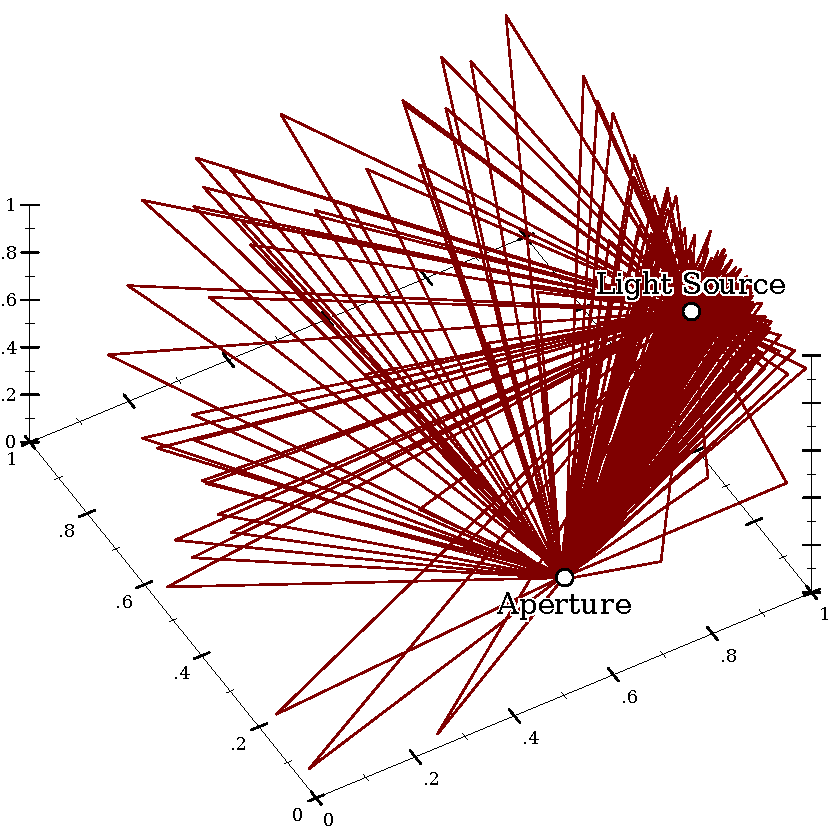
\includegraphics[width=\textwidth]{ray-tracing.pdf}
\end{minipage}
\label{fig:ray-tracing-paths}
}
\tab\ 
\subfloat[Simulated photons constrained to pass through the aperture, projected onto a plane and accumulated.]{
\begin{minipage}{0.43\textwidth}
\centering
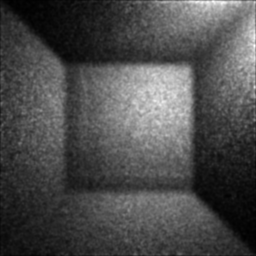
\includegraphics[width=\textwidth]{ray-tracing-projection.png}
\end{minipage}
\label{fig:ray-tracing-projection}
}

\caption[ ]{Ray tracing by constraining the outputs of a probabilistic program.}
\label{fig:ray-tracing}
\end{figure*}

Probabilistic languages that are implemented using advanced Monte Carlo algorithms could be used not just for Bayesian inference, but for \emph{simulating very low-probability events} by encoding the events' criteria as constraints.

Stochastic ray tracing~\cite{cit:veach-1997siggraph-mlt} is one such rare-event simulation task.
As illustrated in \figref{fig:ray-tracing}, to carry out stochastic ray tracing, a probabilistic program simulates a light source emitting a single photon in a random direction, which is reflected or absorbed when it hits a wall.
The program outputs the photon's path, which is constrained to pass through an aperture.
Millions of paths that meet the constraint are sampled, then projected onto a simulated sensor array and accumulated.
The program's main function is recursive:
\begin{equation}
\lzfcsplit{
&simulate!photon~path~dir\ :=\ \\
&\tab \lzfccase{(find!hit~(fst~path)~dir)}{
	reflect~pt~norm & simulate!photon~\pair{pt,path}~(random!half!dir~norm) \\
	absorb~pt & \pair{pt,path}
}
}
\label{eqn:simulate-photon}
\end{equation}
Here, $find!hit$ finds the shape the photon would hit and chooses whether it is reflected or absorbed, and $random!half!dir$ chooses the direction it is reflected.
Running $simulate!photon~\pair{src!pt,\pair{}}~random!dir$ (where $\pair{}$ is the empty list) generates a photon path.
The rest of the program is mostly simple vector math that computes ray-plane intersections.

In contrast, hand-coded stochastic ray tracers, written in general-purpose languages, are much more complex and divorced from the physical processes they simulate, because they must interleave the advanced Monte Carlo algorithms that ensure the aperture constraint is met.

Unfortunately, while many probabilistic programming languages support random real numbers, none are capable of running a probabilistic program like~\eqref{eqn:simulate-photon} under constraints to carry out stochastic ray tracing.
The reason is not lack of engineering or weak algorithms, but is theoretical at its core: they are all either defined or implemented using a naive theory of probability.

While probability mass functions cannot define distributions on $\Re$ that give positive probability to uncountably many values, there is a near-universal substitute that can: probability \emph{density} functions.
Density functions map single values to probability-like quantities, which makes them intuitively appealing and apparently simple.
Unfortunately, density functions are not general enough to be used as probabilistic program meanings without imposing severe limitations on probabilistic languages.
In particular, programs whose outputs are deterministic functions of random values and programs with recursion generally cannot denote density functions.
The program in~\eqref{eqn:simulate-photon} exhibits both characteristics.

Measure-theoretic probability is a more powerful alternative to this naive probability theory based on probability mass and density functions.
It not only subsumes naive probability theory, but is capable of defining any computable probability distribution, and many uncomputable distributions.
But while even the earliest work~\cite{cit:kozen-1979fcs-prob-programs-short} on probabilistic languages is measure-theoretic, the theory's generality has historically made finding useful computational content difficult.

We show that measure-theoretic probability can be made computational by
\begin{enumerate}
	\item Using measure-theoretic probability to define a compositional, denotational semantics that gives a valid denotation to every program.
	\item Deriving an approximating semantics, which allows computing probabilistic conditions under constraints to arbitrary accuracy.
	\item Implementing the approximating semantics and efficiently solving problems.
\end{enumerate}
In fact, our primary implementation, \emph{Dr. Bayes}, produced \figref{fig:ray-tracing-projection} by running a probabilistic program like~\eqref{eqn:simulate-photon} under an aperture constraint.
%Dr. Bayes can be found at \url{https://github.com/ntoronto/drbayes}.

\vspace{0.5\baselineskip}

The rest of this report is organized as follows.
\begin{itemize}
	\item Section~\ref{sec:background} demonstrates why density functions are insufficient for interpreting probabilistic programs. It shows how measure-theoretic probability defines probability distributions using set-valued inverses, or \emph{preimage functions}.
	\item Section~\ref{sec:arrows} presents the categorical tools we use to derive many semantics from a single standard semantics in a way that makes them easy to prove correct.
	\item Section~\ref{sec:nonrecursive-arrows} defines the semantics of nonrecursive, nonprobabilistic programs, which interprets programs as preimage functions.
	\item Section~\ref{sec:recursive-arrows} lifts this semantics to recursive, probabilistic programs.
	\item Section~\ref{sec:approximating-semantics} derives a sound, implementable approximating semantics.
	\item Section~\ref{sec:implementation} describes our implementations and gives examples, including probabilistic verification of floating-point error bounds.
\end{itemize}
In short, we show why and how to run probabilistic programs under constraints by computing preimage functions---that is, by running programs backwards.

\section{Background}
\label{sec:background}

\subsection{Probability Density Functions}

Some distributions of real values can be defined by \keyword{probability density functions}: integrable functions $p : \Re^n \to [0,\infty)$ that integrate to $1$.

The simplest nontrivial probabilistic program is $random$, which returns a uniformly random value in the interval $[0,1]$.
The meaning of $random$ is a probability distribution that can be defined by the density
\begin{equation}
	p : \Re \to [0,\infty)\ \ \ \ \ \ p~x\ :=\
	\begin{cases}
		1 & \text{if } x \in [0,1] \\
		0 & \text{otherwise}
	\end{cases}
\label{eqn:uniform-density}
\end{equation}
Though $p~x$ for any $x$ indicates $x$'s relative frequency, $p~x$ is not a probability.
Probabilities are obtained by integration.
For example, the probability that $random$ returns a value in $[0,0.5]$ is
\begin{equation}
	\int_{0}^{0.5} (p~x)\, \mathit{d}x\ = \
	\int_{0}^{0.5} 1\ \mathit{d}x\ = \
	\Big[x \Big]_{0}^{0.5}\ = \
	0.5 - 0\ = \
	0.5
\end{equation}
Similarly, the probability of $[0.5,0.5]$ or any other singleton set is zero.
In fact, \emph{every} probability density function integrates to zero on singleton sets.

This fact makes it trivial to write a probabilistic program whose distribution cannot be defined by a density.
For example, consider
\begin{equation}
	max~\pair{0.5,random}
\end{equation}
where $max~\pair{a,b}$ returns the greater of the pair $\pair{a,b}$.
This program evaluates to $0.5$ whenever $random$ returns a number in $[0,0.5]$.
In other words, the value of $max~\pair{0.5,random}$ is in $[0.5,0.5]$ with probability $0.5$.
But if its distribution is defined by a density, then $[0.5,0.5]$ must have probability zero---not $0.5$.

A probabilistic language without the $max$ function can still be useful.
It is fairly easy to compute densities for the outputs of single-argument functions that happen to have differentiable inverses, such as exponentiation and square root.
But two-argument functions such as addition and multiplication require evaluating integrals, which generally do not have closed-form solutions.

Perhaps the most constricting limitation of probability density functions is that the number of dimensions must be finite and fixed.
This limitation rules out recursive data types, and makes recursion so difficult that few probabilistic languages attempt to allow it.

\subsection{Measures, and Measures of Preimages}

Measure-theoretic probability gains its expressive power by mapping sets directly to probabilities.
Functions that do so are called \keyword{probability measures}.
For example, the distribution of $random$ is defined by the probability measure
\begin{equation}
	P : \powerset~[0,1] \pto [0,1]\ \ \ \ \ \ P~[a,b]\ =\ b - a
\label{eqn:uniform-measure}
\end{equation}
where $\powerset~[0,1]$ is the powerset of $[0,1]$ and `$\pto$' denotes a partial mapping.
Though~\eqref{eqn:uniform-measure} apparently defines $P$ only on intervals, it is regarded as defining $P$ additionally on countable unions of intervals, their complements, countable unions of such, and so on.
The resulting domain includes almost every subset of $[0,1]$ that can be written down.

Probability measures can be defined on any domain, including domains with variable and infinite dimension.
They can also map singleton sets to nonzero probabilities, which we will demonstrate shortly by deriving a probability measure for $max~\pair{0.5,random}$.

Measure-theoretic probability takes great pains to separate random effects from the pure logic of mathematics.
It does so in the same way Haskell and other purely functional programming languages allow random effects: by interpreting probabilistic processes as \emph{deterministic functions} that operate on an assumed-random source.
The probabilities of sets of outputs are uniquely determined by the probabilities of the corresponding sets of inputs.

Suppose we interpret $max~\pair{0.5,random}$ as the deterministic function
\begin{equation}
	f\ :=\ \fun{r \in [0,1]} max~\pair{0.5,r}
\label{eqn:max-random-manual-interp}
\end{equation}
and assume that $r$ is its uniform random source; i.e. that its distribution is $P$ as defined in~\eqref{eqn:uniform-measure}.
To compute the probability that $max~\pair{0.5,random}$ evaluates to $0.5$, we apply $P$ to the set of all $r$ for which $f~r \in [0.5,0.5]$, and get, as expected,
\begin{equation}
	P~\setb{r \in [0,1]}{f~r \in [0.5,0.5]}\ =\ P~[0,0.5]\ =\ 0.5 - 0\ =\ 0.5
\end{equation}
For any $f$ and $B$, the set $\setb{a \in domain~f}{f~a \in B}$ is called the \keyword{preimage of $B$ under $f$}.
Functions that compute preimages are often denoted $f^{-1}$ to emphasize that they are a sort of generalized inverse function.
However, we find this notation confusing: inverse functions operate on \emph{values} and may not be well-defined, whereas preimage functions operate on \emph{sets} and are \emph{always} well-defined.
We denote $f$'s preimage function by $preimage~f$.
Therefore, the probability that $f$ outputs a value in $B$ is $P~((preimage~f)~B)$, or $P~(preimage~f~B)$.

Though the distribution of $max~\pair{0.5,random}$, or the output of $f$, has no probability density function, its probability measure is defined by
\begin{equation}
	P_f : \powerset~[0.5,1] \pto [0,1]\ \ \ \ \ \ P_f~[a,b]\ =\ P~(preimage~f~[a,b])
\end{equation}
An equivalent, more elegant definition is
\begin{equation}
	P_f\ :=\ P \circ (preimage~f)
\end{equation}
which clearly shows that $P_f$ is factored into a part $P$ that quantifies randomness, and a deterministic part $preimage~f$ that \emph{runs $f$ backwards on sets of outputs}.

This factorization confers the flexibility to interpret probabilistic programs by choosing any $P$ and $f$ for which $P \circ (preimage~f)$ is the correct measure.
For $P$, we choose uniform measures on cartesian products of $[0,1]$ (e.g. $[0,1]^\Nat$) and interpret each $random$ as a projection.
Thus, for the remainder of this paper, we can concentrate solely on computing $preimage~f$.

Because $preimage~f$ is deterministic, techniques to compute it have applications outside of probabilistic programming; for example, constraint-functional languages, type inference, and verification.
More immediately, its determinism means that, for the bulk of this paper, \emph{readers do not need to know anything about probability, let alone measure theory}---only basic set theory.

\subsection{Preimage Semantics}

Several well-known identities suggest that preimages can be computed compositionally, which would make it possible to define a denotational semantics that interprets programs as preimage functions.
For example, we have
\begin{equation}
\begin{aligned}
	preimage~id &\ =\ id
\\
	preimage~(f_2 \circ f_1) &\ =\ (preimage~f_1) \circ (preimage~f_2)
\\
	preimage~\pair{f_1,f_2}~(B_1 \times B_2) &\ =\ (preimage~f_1~B_1) \i (preimage~f_2~B_2)
\end{aligned}
\label{eqn:preimage-identities}
\end{equation}
where $\pair{f_1,f_2} = \fun{a \in (domain~f_1) \i (domain~f_2)} \pair{f_1~a,f_2~a}$ constructs pairing functions and $id$ is the identity function.

It might seem we can easily use identities like those in~\eqref{eqn:preimage-identities} directly to define a semantic function $\meaningof{\cdot}\pre$ that interprets programs as preimage functions.
Unfortunately, our task is not that simple, for the following reasons.
\begin{enumerate}
	\item The $preimage$ function requires its argument to have an observable domain. This includes \keyword{extensional} functions, which are sets of intput/output pairs (i.e. possibly infinite hash tables), but not \keyword{intensional} functions, which are syntactic rules for computing outputs from inputs (e.g. lambdas).\footnote{The lambda $\fun{r} max~\pair{0.5,r}$ is intensional. The notation $\fun{r \in [0,1]} max~\pair{0.5,r}$ constructs an extensional function by applying $\fun{r} max~\pair{0.5,r}$ to every value in $[0,1]$.}
\label{problem:observable-domain}
	\item We must ensure $preimage~f~B$ is always in the domain of the chosen probability measure $P$. (Recall that probability measures are partial functions.) If this is true, we say $f$ is \keyword{measurable}. Proving measurability is difficult, especially if $f$ may not terminate.%
\label{problem:measurability}
	\item The function $app : (X \to Y) \times X \to Y$, when restricted to measurable functions, is not generally measurable, if we want good approximation properties~\cite{cit:aumann-1961ijm-borel}. This makes interpreting higher-order application difficult.%
\label{problem:higher-orderness}
\end{enumerate}
Implementing a language based on preimage semantics is complicated because
\begin{enumerate}
	\setcounter{enumi}{3}
	\item Ordinary set-based mathematics is unlike any implementation language.%
\label{problem:different-language}
	\item It requires running programs written in a Turing-equivalent language backwards, efficiently, on possibly uncountable sets of outputs.%
\label{problem:backward-efficient}
\end{enumerate}

We address~\ref{problem:observable-domain} and~\ref{problem:different-language} by developing our semantics using \lzfclang~\cite{cit:toronto-2012flops-lzfc}, an untyped, call-by-value $\lambda$-calculus with infinite sets, real numbers, extensional functions such as $\fun{r \in [0,1]} max~\pair{0.5,r}$, intensional functions such as $\fun{r} max~\pair{0.5,r}$, a computable sublanguage, and an operational semantics.
It is essentially ordinary mathematics extended with lambdas and general recursion, or equivalently a lambda calculus extended with uncountably infinite sets and set operations.

We have addressed difficulty~\ref{problem:measurability} by proving that all programs' interpretations as functions are measurable if language primitives are measurable, including uncomputable primitives such as limits and real equality, regardless of nontermination.
The proof interprets programs as extensional functions and applies well-known theorems from measure theory (such as the identities in~\eqref{eqn:preimage-identities}).
Unfortunately, the required machinery does not fit in this report; see the first author's dissertation~\cite{cit:toronto-thesis} for the entire development.

We avoid difficulty~\ref{problem:higher-orderness} for now by interpreting a language with \emph{first-order} functions and recursion.

We address~\ref{problem:backward-efficient} by deriving and implementing a \emph{conservative approximation} of the preimage semantics, and using its approximations to compute measures of preimages with arbitrary accuracy.

\subsection{Nonstandard Abstract Interpretation, Categorically}

\todo{David: Need a transition from previous subsection.}

\todo{David: Need some forward-looking intuition about why you need the following.}

We interpret nonrecursive, nonprobabilistic programs three different ways, using
\begin{enumerate}
	\item A \keyword{standard semantics} $\meaningof{\cdot}_\bot$ that interprets programs that may raise errors (e.g. divide-by-zero) as functions.
	\item A \keyword{nonstandard semantics} $\meaningof{\cdot}\pre$ that interprets programs as preimage functions, which operate on uncountable sets, and are thus unimplementable.
	\item An \keyword{approximating semantics} $\meaningof{\cdot}\pre'$ that interprets programs as \emph{approximating} preimage functions, which \emph{are} implementable.
\end{enumerate}
Of course, we must prove for any program $\mathit{p}$, that $\meaningof{\mathit{p}}\pre$ correctly computes preimages under $\meaningof{\mathit{p}}_\bot$, and that $\meaningof{\mathit{p}}\pre'$ is sound with respect to $\meaningof{\mathit{p}}\pre$.

\todo{David: Put hats on approximating or approximate things.}

For recursive, probabilistic programs, we define three more semantic functions analogous to $\meaningof{\cdot}_\bot$, $\meaningof{\cdot}\pre$ and $\meaningof{\cdot}\pre'$, that have analogous proof obligations.
We also prove that they correctly interpret nonrecursive, nonprobabilistic programs.

In the full development~\cite{cit:toronto-thesis}, two more semantic functions interpret programs as extensional functions, which are used to prove measurability.
Another semantic function collects information needed for advanced Monte Carlo algorithms.

In all, we have 9 related semantic functions, each defined by 11 or 12 rules, whose correctness and relationships must be proved by structural induction.
Doing so is tedious and error-prone.
We need a way to parameterize one semantic function on many meanings, where each ``meaning'' is simpler than a semantic function and ideally has exploitable properties.

Moggi~\cite{cit:moggi-1989lics-monads} introduced monads as a categorical ``metalanguage'' for interpreting programs.
Wadler~\cite{cit:wadler-2001-monads} showed how to use monad categories in pure functional programming to encode and hide side effects such as mutation and randomness.
Haskell programmers now primarily encode programs with side effects using \keyword{do-notation}, which is transformed into any monad.
Essentially, Haskell has a built-in semantic function parameterized on a monad.

Other researchers have identified arrows~\cite{cit:hughes-2000scp-arrows} and idioms~\cite{cit:mcbride-2008jfp-idiom} as useful kinds of categories.
Different kinds of categories are good for encoding different kinds of effects, and have different levels of expressiveness~\cite{cit:lindley-2008entcs-idiom-arrow-monad}.
Arrows are good categories for interpreting first-order languages.
We therefore interpret programs 9 different ways by parameterizing a semantic function on one of 9 arrow categories.

\todo{David: It might be worth giving a graphical figure presenting these semantics and the relations between them. I have a hard time seeing why you need so many variations.}

In our formulation, an arrow category consists of a type constructor and five combinators; each is thus half as complicated as the semantic function.
Their categorical properties also allow two drastic simplifications.
First, they allow proving the correctness of one semantic function with respect to another by proving a simple theorem about their arrows.
Second, they allow us to \emph{derive} all the arrows for recursive, probabilistic programs from the arrows for nonrecursive, nonprobabilistic programs, by defining one function and proving one theorem.

\subsection{Types and Notation}

Because some arrows carry out uncountably infinite computations, we must define their combinators in a sufficiently powerful $\lambda$-calculus.
We use \lzfclang~\cite{cit:toronto-2012flops-lzfc}.

Though \lzfclang is untyped, it helps to use an auxiliary type system.
Types are manually checked, polymorphic, and characterized by these rules:
\begin{itemize}
	\item A free type variable is universally quantified; if uppercase, it denotes a set.
	\item A set denotes a member of that set.
	\item $x \to y$ denotes an intensional or extensional partial function.
	\item $\pair{x,y}$ denotes a pair of values with types $x$ and $y$.
	\item $Y^X$ denotes a vector of $Y$ indexed by $X$: a total, extensional function $X \to Y$.
	\item $Set~x$ denotes a set with members of type $x$.
\end{itemize}
Because the type $Set~X$ denotes the same values as the set $\powerset~X$ (i.e. subsets of the set $X$) we regard them as equivalent.
Similarly, $\pair{X,Y}$ is equivalent to $X \times Y$.

Examples of types are those of the \lzfclang primitives membership $(\in) : x \to Set~x \to Bool$, powerset $\powerset : Set~x \to Set~(Set~x)$, big union $\U : Set~(Set~x) \to Set~x$, and the \texttt{map}-like $image : (x \to y) \to Set~x \to Set~y$.

We use adjacency (i.e. $f~a$) for all function application, including extensional functions.
For example, if $f : [0,1]^\Nat$, then $f$ is a countable vector of reals in $[0,1]$ (a total, extensional function from $\Nat$ to $[0,1]$), and $f~0$ is its first element.

We elide proofs to save space.
The full proofs can be found in the first author's dissertation~\cite{cit:toronto-thesis}.

%%%%%%%%%%%%%%%%%%%%%%%%%%%%%%%%%%%%%%%%%%%%%%%%%%%%%%%%%%%%%%%%%%%%%%%%%%%%%%%%%%%%%%%%%%%%%%%%%%%%%
%%%%%%%%%%%%%%%%%%%%%%%%%%%%%%%%%%%%%%%%%%%%%%%%%%%%%%%%%%%%%%%%%%%%%%%%%%%%%%%%%%%%%%%%%%%%%%%%%%%%%
%%%%%%%%%%%%%%%%%%%%%%%%%%%%%%%%%%%%%%%%%%%%%%%%%%%%%%%%%%%%%%%%%%%%%%%%%%%%%%%%%%%%%%%%%%%%%%%%%%%%%

\section{Arrows and First-Order Semantics}
\label{sec:arrows}

Arrows~\cite{cit:hughes-2000scp-arrows}, like monads~\cite{cit:wadler-2001-monads}, thread effects through computations in a way that imposes structure.
But arrow computations are always
\begin{enumerate}
	\item Function-like. The type constructor for arrow $a$ is written $x \arrow_a y$ to connote this. In fact, the \keyword{function arrow}'s type constructor is $x \arrow y ::= x \to y$.
	\item First-order. There is no way to derive the higher-order application combinator $app : \pair{x \arrow_a y, x} \arrow_a y$ from the combinators that define arrow $a$.
\end{enumerate}
The first property makes arrows a good fit for a compositional translation from expressions to pure functions that operate on random sources.
The second property makes arrows a good fit for the semantics of a first-order language.

\subsection{Arrow Categories and Laws}
\label{sec:arrow-definitions}

Using arrows factors a first-order program's computations into
\begin{enumerate}
	\item Referring to primitive functions.
	\item Applying primitive or first-order functions.
	\item Binding values to local variables and creating data structures.
	\item Branching based on the results of prior computations.
\end{enumerate}
The first four arrow combinators correspond respectively with each of these tasks.
The last combinator allows lazy branching in a call-by-value language.

\newcommand{\arrowfootnote}{These are actually arrows \emph{with choice}, which are typically defined using $first_a$ and $left_a$ instead of $(\arrowpair_a)$ and $\arrowif_a$.
We find $\arrowif_a$ more natural for semantics than $left_a$, and $(\arrowpair_a)$ better matches the pairing preimage identity in~\eqref{eqn:preimage-identities}.}

\begin{definition}[arrow\footnote{\arrowfootnote}]Let $1 := \set{0}$. A binary type constructor $(\arrow\gen)$ and
\begin{displaybreaks}
\begin{equation*}
\begin{aligned}
	\arrowarr\gen &: (x \to y) \to (x \arrow\gen y)
		& \text{\emph{lift}}
\nobreak\\
	(\arrowcomp\gen) &: (x \arrow\gen y) \to (y \arrow\gen z) \to (x \arrow\gen z)
		& \text{\emph{compose}}
\\
	(\arrowpair\gen) &: (x \arrow\gen y) \to (x \arrow\gen z) \to (x \arrow\gen \pair{y,z})
		& \text{\emph{pair}}
\\
	\arrowif\gen &: (x \arrow\gen Bool) \to (x \arrow\gen y) \to (x \arrow\gen y) \to (x \arrow\gen y)
		\tab\tab& \text{\emph{if-then-else}}
\nobreak\\
	\arrowlazy\gen &: (1 \to (x \arrow\gen y)) \to (x \arrow\gen y)
		& \text{\emph{laziness}}
\label{eqn:arrow-combinators}
\end{aligned}
\end{equation*}
\end{displaybreaks}
define an \keyword{arrow} if certain monoid, homomorphism, and structural laws hold.
\end{definition}

For example, the function arrow is defined by the type constructor $x \arrow y ::= x \to y$ and the combinators
\begin{equation}
\begin{aligned}
	\arrowarr~f &\ := \ f \\
	(f_1~\arrowcomp~f_2)~a &\ := \ f_2~(f_1~a) \\
	(f_1~\arrowpair~f_2)~a &\ := \ \pair{f_1~a,f_2~a} \\
	\arrowif~f_1~f_2~f_3~a &\ := \ if~(f_1~a)~(f_2~a)~(f_3~a) \\
	\arrowlazy~f~a &\ :=\ f~0~a
\end{aligned}
\label{eqn:function-arrow}
\end{equation}
Suppose we want to use the function arrow to interpret the probabilistic program $max~\pair{0.5,random}$ as a deterministic function that operates on a random source $r$.
To do so compositionally, we must interpret every subexpression as a deterministic function.
For any random source $r$, the interpretation of $0.5$ should return $0.5$; it is therefore $\fun{r}0.5$.
If we assume $r \in [0,1]$, then the interpretation of $random$ is $\fun{r} r$, or $id$.
We can use $(\arrowpair)$ to apply each of these interpretations to the random source to create a pair, and $(\arrowcomp)$ to send the pair to $max$.

The interpretation of $max~\pair{0.5,random}$ is thus
\begin{equation}
\begin{aligned}
	((\fun{r}0.5)~\arrowpair~id)~\arrowcomp~max
	&\ \equiv\ (\fun{r} \pair{(\fun{r}0.5)~r,id~r})~\arrowcomp~max
	\tab && \textrm{def. of $(\arrowpair)$}
\\
	&\ \equiv\ (\fun{r} \pair{0.5,r})~\arrowcomp~max
	&& \textrm{$\beta$ reduce}
\\
	&\ \equiv\ \fun{r} max~((\fun{r} \pair{0.5,r})~r)
	&& \textrm{def. of $(\arrowcomp)$}
\\
	&\ \equiv\ \fun{r} max~\pair{0.5,r}
	&& \textrm{$\beta$ reduce}
\end{aligned}
\end{equation}
which is equivalent to our manual interpretation of $max~\pair{0.5,random}$ in~\eqref{eqn:max-random-manual-interp}.

Only the function arrow can so cavalierly use pure functions as arrow computations.
In any other arrow $a$, pure functions must be \emph{lifted} using $\arrowarr_a$, to allow the arrow to manage any state or effects.
Assuming the random source is a single value in $[0,1]$, the interpretation of $max~\pair{0.5,random}$ in any arrow $a$ is thus
\begin{equation}
	(arr_a~(\fun{r}0.5)~\arrowpair_a~arr_a~id)~\arrowcomp_a~arr_a~max
\end{equation}


So far, we have ignored the many arrow laws, which ensure that effects are correctly ordered, and are occasionally useful in proofs.
Fortunately, we can prove them all for an arrow by defining it in terms of another for which the laws hold, and proving two properties.
The first is a distributive property.

\begin{definition}[arrow homomorphism]
\label{def:arrow-homomorphism}
$lift\genb : (x \arrow\gen y) \to (x \arrow\genb y)$ is an \mykeyword{arrow homomorphism} from arrow $\mathrm{a}$ to arrow $\mathrm{b}$ if these distributive laws hold:
\begin{displaybreaks}
\begin{align}
	lift\genb~(\arrowarr\gen~f) &\ \equiv \ \arrowarr\genb~f
	\label{eqn:lift-distributes-over-arr}
\nobreak\\
	lift\genb~(f_1~\arrowcomp\gen~f_2) &\ \equiv \ (lift\genb~f_1)~\arrowcomp\genb~(lift\genb~f_2)
	\label{eqn:lift-distributes-over-comp}
\\
	lift\genb~(f_1~\arrowpair\gen~f_2) &\ \equiv \ (lift\genb~f_1)~\arrowpair\genb~(lift\genb~f_2)
	\label{eqn:lift-distributes-over-pair}
\\
	\arrowlift\genb~(\arrowif\gen~f_1~f_2~f_3) &\ \equiv \ 
		\arrowif\genb~(lift\genb~f_1)~(lift\genb~f_2)~(lift\genb~f_3)
	\label{eqn:lift-distributes-over-if}
\nobreak\\
	\arrowlift\genb~(\arrowlazy\gen~f) &\ \equiv \
		\arrowlazy\genb~\fun{0}{\arrowlift\genb~(f~0)}
	\label{eqn:lift-distributes-over-lazy}
\end{align}
where ``$\equiv$'' is an arrow-specific equivalence relation.
\end{displaybreaks}
\end{definition}

\begin{theorem}[right-invertible homomorphism implies arrow laws]
\label{thm:arrow-epimorphism}
If $\arrowlift\genb : (x \arrow\gen y) \to (x \arrow\genb y)$ is a homomorphism from arrow $a$ to arrow $b$ and has a right inverse, and the combinators of $a$ obey the arrow laws, then the combinators of $b$ obey the arrow laws.
\end{theorem}
\begin{proof}
For each law, substitute right inverses, factor out $\arrowlift\genb$, apply law for arrow $a$, distribute $\arrowlift\genb$, and cancel right inverses.
\qed
\end{proof}

%Arrow homomorphisms are important for more than proving arrow laws.
%After we define a semantic function parameterized on arrows, we will be able to derive new semantics from old in a way that proves them correct almost for free, simply by defining an arrow homomorphism.

\subsection{First-Order Let-Calculus Semantics}

\begin{figure*}[!tb]\centering
\smallmathfont
\begin{align*}
	\mathit{p} &\ ::\equiv \ \mathit{x := e};\ ...\ ; \mathit{e}
\\
	\mathit{e} &\ ::\equiv \ \mathit{x~e}\ |\ let~\mathit{e~e}\ |\ env~\mathit{n}\ |\ \mathit{\pair{e,e}}\ |\ fst~\mathit{e}\ |\ snd~\mathit{e}\ |\ if~\mathit{e~e~e}\ |\ \mathit{v}
\\
	\mathit{v} &\ ::\equiv \ \text{[first-order constants]}
\\[-6pt]
\end{align*}
\begin{align*}
\begin{aligned}[t]
	\meaningof{\mathit{x} := \mathit{e};\ ...\ ; \mathit{e_b}}\gen &\ :\equiv\
		\mathit{x} := \meaningof{\mathit{e}}\gen;\ ...\ ; \meaningof{\mathit{e_b}}\gen
\\[3pt]
	\meaningof{\mathit{x}~\mathit{e}}\gen &\ :\equiv\
		\meaningof{\pair{\mathit{e},\pair{}}}\gen~\arrowcomp\gen~\mathit{x}
\\
	\meaningof{\pair{\mathit{e}_1,\mathit{e}_2}}\gen &\ :\equiv\
		\meaningof{\mathit{e}_1}\gen~\arrowpair\gen~\meaningof{\mathit{e}_2}\gen
\\
	\meaningof{fst~\mathit{e}}\gen &\ :\equiv\
		\meaningof{\mathit{e}}\gen~\arrowcomp\gen~\arrowarr\gen~fst
\\
	\meaningof{snd~\mathit{e}}\gen &\ :\equiv\
		\meaningof{\mathit{e}}\gen~\arrowcomp\gen~\arrowarr\gen~snd
\\
	\meaningof{\mathit{v}}\gen &\ :\equiv\ \arrowarr\gen~(const~\mathit{v})
\\[6pt]
	id &\ := \ \fun{a} a
\\
	const~b &\ := \ \fun{a} b
\\
\end{aligned}
&\tab\tab\ 
\begin{aligned}[t]
\\[3pt]
	\meaningof{let~\mathit{e}~\mathit{e_b}}\gen &\ :\equiv\ 
		(\meaningof{\mathit{e}}\gen~\arrowpair\gen~\arrowarr\gen~id)~
			\arrowcomp\gen~
		\meaningof{\mathit{e_b}}\gen
\\
	\meaningof{env~0}\gen &\ :\equiv\ \arrowarr\gen~fst
\\
	\meaningof{env~(\mathit{n}+1)}\gen &\ :\equiv\ \arrowarr\gen~snd~\arrowcomp\gen~\meaningof{env~\mathit{n}}\gen
\\
	\meaningof{if~\mathit{e_c}~\mathit{e_t}~\mathit{e_f}}\gen &\ :\equiv\
		\arrowif\gen~
			\meaningof{\mathit{e_c}}\gen~
			\meaningof{lazy~\mathit{e_t}}\gen~
			\meaningof{lazy~\mathit{e_f}}\gen
\\
	\meaningof{lazy~\mathit{e}}\gen &\ :\equiv\ \arrowlazy\gen~\fun{0}{\meaningof{\mathit{e}}\gen}
\\
\\
	\text{subject to} &\ \meaningof{\mathit{p}}\gen : \pair{} \arrow\gen y \ \text{for some $y$}
\end{aligned}
\end{align*}
\bottomhrule
\caption[ ]{Interpretation of a let-calculus with first-order definitions and De-Bruijn-indexed bindings as arrow $\mathrm{a}$ computations.
}
\label{fig:semantic-function}
\end{figure*}

Figure~\ref{fig:semantic-function} defines a semantic function $\meaningof{\cdot}\gen$ that interprets first-order programs as arrow computations for any arrow $a$.
A program is a sequence of definition statements followed by a final expression.
Functions are named, but local variables and arguments are not.
Instead, variables are referred to by De Bruijn indexes, with $0$ referring to the innermost binding.

We call this style of interpretation \mykeyword{stack-passing style}.
The final expression has type $\pair{} \arrow\gen y$, where $y$ is the type of the program's output and $\pair{}$ denotes the empty stack.
A $let$ expression uses pairing $(\arrowpair\gen)$ to push a value onto the stack and composition $(\arrowcomp\gen)$ to pass the resulting stack to its body.
First-order functions have type $\pair{x,\pair{}} \arrow\gen y$ where $x$ is the argument type and $y$ is the return type.
Application passes a stack with just an $x$ using pairing and composition.

We regard programs as if they were their final expressions; therefore statements about ``all expressions $\mathit{e}$'' such as the following apply to all programs $\mathit{p}$.

\begin{definition}[well-defined expression]
\label{def:well-defined-expression}
An expression $\mathit{e}$ is \keyword{well-defined} under arrow $a$ if $\meaningof{\mathit{e}}\gen : x \arrow\gen y$ for some $x$ and $y$, and $\meaningof{\mathit{e}}\gen$ terminates.
\end{definition}

From here on, we assume all expressions are well-defined.
(The arrow $a$ will be clear from context.)
Well-definedness does not guarantee that \emph{running} an interpretation terminates.
It just simplifies statements about expressions, such as the following theorem, on which most of our semantic correctness results rely.

\begin{theorem}[homomorphisms distribute over expressions]
\label{thm:homomorphism-implies-correct}
Let $\arrowlift\genb : (x \arrow\gen y) \to (x \arrow\genb y)$ be an arrow homomorphism.
For all $\mathit{e}$, $\meaningof{\mathit{e}}\genb \equiv \arrowlift\genb~\meaningof{\mathit{e}}\gen$.%
\end{theorem}
\begin{proof}
By structural induction and homomorphism properties~\eqref{eqn:lift-distributes-over-arr}--\eqref{eqn:lift-distributes-over-lazy}.
\qed
\end{proof}

Much of our development proceeds in the following way.
\begin{enumerate}
	\item Define a simple arrow $a$ to interpret programs using $\meaningof{\cdot}_a$.
	\item Define $\arrowlift\genb : (x \arrow\gen y) \to (x \arrow\genb y)$ from arrow $a$ to arrow $b$ for which $\arrowlift\genb~f$ for any $f : x \arrow_a y$ is obviously correct.
	\item Prove $lift_b$ is a homomorphism; therefore $\meaningof{\mathit{e}}\genb$ is correct (Theorem~\ref{thm:homomorphism-implies-correct}).
	\item Prove $lift_b$ is right-invertible; therefore $b$ obeys the arrow laws (Theorem~\ref{thm:arrow-epimorphism}).
\end{enumerate}
In shorter terms, \emph{if arrow $b$ is defined in terms of a right-invertible homomorphism from $a$ to $b$, then $\meaningof{\cdot}_b$ is correct with respect to $\meaningof{\cdot}_a$}.

%%%%%%%%%%%%%%%%%%%%%%%%%%%%%%%%%%%%%%%%%%%%%%%%%%%%%%%%%%%%%%%%%%%%%%%%%%%%%%%%%%%%%%%%%%%%%%%%%%%%%
%%%%%%%%%%%%%%%%%%%%%%%%%%%%%%%%%%%%%%%%%%%%%%%%%%%%%%%%%%%%%%%%%%%%%%%%%%%%%%%%%%%%%%%%%%%%%%%%%%%%%
%%%%%%%%%%%%%%%%%%%%%%%%%%%%%%%%%%%%%%%%%%%%%%%%%%%%%%%%%%%%%%%%%%%%%%%%%%%%%%%%%%%%%%%%%%%%%%%%%%%%%

\section{The Bottom and Preimage Arrows}
\label{sec:nonrecursive-arrows}

\newcommand{\youarehere}[1]%
{%
\begin{equation}%
\begin{CD}%
X \botto Y   @>\liftpre>>   X \preto Y \\%
@V{\eta_\pbot}VV              @VV{\eta\ppre}V\\%
X \pbotto Y  @>>\liftppre>  X \ppreto Y%
\end{CD}%
\label{#1}%
\end{equation}%
}

The following commutative diagram shows the relationships between the exact arrows we define.
We will use it as a sort of roadmap.
\youarehere{eqn:roadmap-diagram2}
In this section, we define the top row, which are the exact arrows for interpreting nonrecursive, nonprobabilistic programs.

\subsection{The Bottom Arrow}

\begin{figure*}[!tb]\centering
\smallmathfont
\begin{align*}
\begin{aligned}[t]
	&X \botto Y \ ::= \ X \to Y_\bot
\\[0.5\baselineskip]
	&\arrbot~f~a \ := \ f~a
\\
	&(f_1~\compbot~f_2)~a \ := \
		\lzfccase{f_1~a}{
			\bot & \bot \\
			b & f_2~b}
\\
	&(f_1~\pairbot~f_2)~a \ := \ 
	\lzfccase{\pair{f_1~a,f_2~a}}{
		\pair{\bot,\uscore} & \bot \\
		\pair{\uscore,\bot} & \bot \\
		\pair{b_1,b_2} & \pair{b_1,b_2}}
\end{aligned}
&\tab\tab\tab
\begin{aligned}[t]
	&\ifbot~f_1~f_2~f_3~a \ := \ 
		\lzfccase{f_1~a}{true & f_2~a \\ false & f_3~a \\ \bot & \bot}
\\
	&\lazybot~f~a \ := \ f~0~a
\end{aligned}
\end{align*}
\bottomhrule
\caption[ ]{Bottom arrow definitions.}
\label{fig:bottom-arrow-defs}
\end{figure*}

To use Theorem~\ref{thm:homomorphism-implies-correct} to prove correct the interpretations of expressions as preimage arrow computations, we need to define the preimage arrow in terms of a simpler arrow with easily understood behavior.
The function arrow~\eqref{eqn:function-arrow} is an obvious candidate.
However, we will need to explicitly handle nontermination as an error value, so we need a slightly more complicated arrow.

\figref{fig:bottom-arrow-defs} defines the \mykeyword{bottom arrow}, which is similar to the function arrow but propagates the error value $\bot$.
Its computations have type $X \botto Y ::= X \to Y_\bot$, where $Y_\bot ::= Y \u \set{\bot}$.

To prove the arrow laws, we need coarse enough notion of equivalence.

\begin{definition}[bottom arrow equivalence]
Two computations $f_1 : X \botto Y$ and $f_2 : X \botto Y$ are equivalent, or $f_1 \equiv f_2$, when $f_1~a = f_2~a$ for all $a \in X$.
\end{definition}

Using bottom arrow equivalence, it is easy to show that $(\botto)$ is isomorphic to the Maybe monad's Kleisli arrow.
By Theorem~\ref{thm:arrow-epimorphism}, the arrow laws hold.

\subsection{The Preimage Function Type and Operations}
\label{sec:lazy-preimage-mappings}

\begin{figure*}[!tb]\centering
\smallmathfont
\begin{align*}
&\begin{aligned}[t]
	&\begin{aligned}[t]
		&X \prepto Y ::= \pair{Set~Y, Set~Y \to Set~X}
	\end{aligned} \\
\\[-6pt]
	&\begin{aligned}[t]
		&pre : (X \botto Y) \to (X \prepto Y) \\
		&\lzfcsplit{&pre~f~A \ := \ \pair{image_\bot~f~A, preimage_\bot~f~A}}
	\end{aligned} \\
\\[-6pt]
	&\begin{aligned}[t]
		&\emptyset\pre \ := \ \pair{\emptyset,\fun{B} \emptyset}
	\end{aligned} \\
\\[-6pt]
	&\begin{aligned}[t]
		&ap\pre : (X \prepto Y) \to Set~Y \to Set~X \\
		&ap\pre~\pair{Y',p}~B \ := \ p~(B \i Y') 
	\end{aligned} \\
\\[-6pt]
	&\begin{aligned}[t]
		&range\pre : (X \prepto Y) \to Set~Y \\
		&range\pre~\pair{Y',p} \ := \ Y'
	\end{aligned}
\end{aligned}
&&\begin{aligned}[t]
	&\begin{aligned}[t]
		&\pair{\cdot,\cdot}\pre : (X \prepto Y_1) \to (X \prepto Y_2) \to (X \prepto Y_1 \times Y_2) \\
		&\pair{\pair{Y_1',p_1},\pair{Y_2',p_2}}\pre \ := \ \\
		&\tab\lzfclet{
			Y' & Y_1' \times Y_2' \\
			p & \fun{B}{\U\limits_{\pair{b_1,b_2} \in B}(p_1~\set{b_1}) \i (p_2~\set{b_2})} \\
		}{\pair{Y',p}}
	\end{aligned} \\
\\[-6pt]
	&\begin{aligned}[t]
		&(\circ\pre) : (Y \prepto Z) \to (X \prepto Y) \to (X \prepto Z) \\
		&\pair{Z',p_2} \circ\pre h_1 \ := \ \pair{Z', \fun{C}{ap\pre~h_1~(p_2~C)}}
	\end{aligned} \\
\\[-6pt]
	&\begin{aligned}[t]
		&(\u\pre) : (X \prepto Y) \to (X \prepto Y) \to (X \prepto Y) \\
		&\lzfcsplit{
			&h_1 \u\pre h_2 \ := \ 
			\lzfclet{
					Y' & (range\pre~h_1) \u (range\pre~h_2) \\
					p & \fun{B}{(ap\pre~h_1~B) \u (ap\pre~h_2~B)}
				}{\pair{Y',p}}
		}
	\end{aligned}
\end{aligned}
\\[-6pt]
&\begin{aligned}[t]
\hline
\\[-8pt]
	&\begin{aligned}[t]
		&image_\bot : (X \botto Y) \to Set~X \to Set~Y \\
		&image_\bot~f~A \ := \ (image~f~A) \w \set{\bot}
	\end{aligned}
\end{aligned}
&&\begin{aligned}[t]
\hline
\\[-8pt]
	&\begin{aligned}[t]
		&preimage_\bot : (X \botto Y) \to Set~X \to Set~Y \to Set~X \\
		&preimage_\bot~f~A~B \ := \ \setb{a \in A}{f~a \in B}
	\end{aligned}
\end{aligned}
\end{align*}
\bottomhrule
\caption[ ]{Preimage functions and operations.}
\label{fig:preimage-mapping-defs}
\end{figure*}

Before defining the preimage arrow, we need a type of preimage functions.
$Set~Y \to Set~X$ would be a good candidate, except that the $(\comppre)$ combinator will require preimage functions to have observable domains, but instances of $Set~Y \to Set~X$ may be intensional functions.
We therefore define
\begin{equation}
	X \prepto Y \ ::= \ \pair{Set~Y, Set~Y \to Set~X}
\end{equation}
as the type of preimage functions.
\figref{fig:preimage-mapping-defs} defines the necessary operations on them.
Operations $\pair{\cdot,\cdot}\pre$ and $(\circ\pre)$ return preimage functions that compute preimages under pairing and composition, and are derived from the identities in~\eqref{eqn:preimage-identities}; $(\u\pre)$ computes unions and is used to define $\ifpre$.

\figref{fig:preimage-mapping-defs} also defines $image_\bot$ and $preimage_\bot$ to operate on bottom arrow computations: $image_\bot~f~A$ computes $f$'s range (with domain $A$), and $preimage_\bot~f~A$ returns a function that computes preimages under $f$ restricted to $A$.
Together, they can be used to convert bottom arrow computations to preimage functions:
\begin{equation}
\begin{aligned}
	&pre : (X \botto Y) \to Set~X \to (X \prepto Y) \\
	&pre~f~A \ := \ \pair{image_\bot~f~A, preimage_\bot~f~A}
\end{aligned}
\end{equation}
Lastly, the $ap\pre$ function in \figref{fig:preimage-mapping-defs} applies a preimage function to a set.

Preimage arrow correctness depends on $ap\pre$ and $pre$ behaving like $preimage_\bot$.

\begin{theorem}[$ap\pre$ of $pre$ computes preimages]
\label{thm:pre-like-preimage}
Let $f : X \botto Y$. For all $A \subseteq X$ and $B \subseteq Y$, $ap\pre~(pre~f~A)~B = preimage_\bot~f~A~B$.
\end{theorem}
\begin{proof}
Expand definitions; use basic facts about $(\w)$, $(\i)$ and $image$.
\qed
\end{proof}

\subsection{The Preimage Arrow}
\label{sec:preimage-arrow}

\begin{figure*}[!tb]\centering
\smallmathfont
\begin{align*}
\begin{aligned}[t]
	X \preto Y &\ ::=\ Set~X \to (X \prepto Y)
\\[0.5\baselineskip]
	\arrpre &\ := \ \liftpre \circ \arrbot
\\
	(h_1~\comppre~h_2)~A &\ := \ 
		\lzfclet{
			h_1' & h_1~A \\
			h_2' & h_2~(range\pre~h_1')
		}{h_2' \circ\pre h_1'}
\\
	(h_1~\pairpre~h_2)~A &\ := \ \pair{h_1~A,h_2~A}\pre
\end{aligned}
&\tab\tab\tab
\begin{aligned}[t]
	&\lzfcsplit{&\ifpre~h_1~h_2~h_3~A \ := \ \\
		&\tab\lzfclet{
			h_1' & h_1~A \\
			h_2' & h_2~(ap\pre~h_1'~\set{true}) \\
			h_3' & h_3~(ap\pre~h_1'~\set{false})
		}{h_2' \u\pre h_3'}}
\\
	&\lazypre~h~A \ := \ if~(A = \emptyset)~\emptyset\pre~(h~0~A)
\\
	&\liftpre \ := \ pre
\end{aligned}
\end{align*}
\bottomhrule
\caption[ ]{Preimage arrow definitions.}
\label{fig:preimage-arrow-defs}
\end{figure*}

If we define the \mykeyword{preimage arrow} type constructor as
\begin{equation}
	X \preto Y \ ::= \ Set~X \to (X \prepto Y)
\end{equation}
then we already have a lift $\liftpre : (X \botto Y) \to (X \preto Y)$ from the bottom arrow to the preimage arrow: $pre$.
If $\liftpre$ is $pre$, then by Theorem~\ref{thm:pre-like-preimage}, lifted bottom arrow computations compute correct preimages, exactly as we should expect them to.

\figref{fig:preimage-arrow-defs} defines the preimage arrow in terms of the preimage function operations in \figref{fig:preimage-mapping-defs}.
For these definitions to make $\liftpre$ a homomorphism, preimage arrow equivalence must mean ``computes the same preimages.''

\begin{definition}[preimage arrow equivalence]
Two preimage arrow computations $h_1 : X \preto Y$ and $h_2 : X \preto Y$ are equivalent, or $h_1 \equiv h_2$, when 
$ap\pre~(h_1~A)~B = ap\pre~(h_2~A)~B$ for all $A \subseteq X$ and $B \subseteq Y$.
\end{definition}

\begin{theorem}[preimage arrow correctness]
$\liftpre$ is a homomorphism.
\end{theorem}

\begin{corollary}[semantic correctness]
\label{cor:preimage-arrow-correctness}
For all $\mathit{e}$, $\meaningof{\mathit{e}}\pre \equiv \liftpre~\meaningof{\mathit{e}}_\bot$.
\end{corollary}

In other words, $\meaningof{\mathit{e}}\pre$ always computes correct preimages under $\meaningof{\mathit{e}}_\bot$.

The type $X \preto Y$ does not constrain its inhabitants to behave intuitively; e.g.
\begin{equation}
\begin{aligned}
	&unruly : Bool \preto Bool \\
	&unruly~A \ := \ \pair{Bool \w A, \fun{B} B}
\end{aligned}
\end{equation}
So $ap\pre~(unruly~\set{true})~\set{false} = \set{false} \i (Bool \w \set{true}) = \set{false}$---a ``preimage'' that does not even intersect the given domain $\set{true}$.
Other examples show that preimage computations are not necessarily monotone, and lack other desirable properties.
Those with desirable properties obey the following law.

\begin{definition}[preimage arrow law]
\label{def:preimage-arrow-law}
Let $h : X \preto Y$. If there exists an $f : X \botto Y$ such that $h \equiv \liftpre~f$, then $h$ obeys the \mykeyword{preimage arrow law}.
\end{definition}

By homomorphism of $\liftpre$, preimage arrow combinators preserve the preimage arrow law.
From here on, we assume all $h : X \preto Y$ obey it.
By Definition~\ref{def:preimage-arrow-law}, $\liftpre$ has a right inverse; by Theorem~\ref{thm:arrow-epimorphism}, the arrow laws hold.

%%%%%%%%%%%%%%%%%%%%%%%%%%%%%%%%%%%%%%%%%%%%%%%%%%%%%%%%%%%%%%%%%%%%%%%%%%%%%%%%%%%%%%%%%%%%%%%%%%%%%
%%%%%%%%%%%%%%%%%%%%%%%%%%%%%%%%%%%%%%%%%%%%%%%%%%%%%%%%%%%%%%%%%%%%%%%%%%%%%%%%%%%%%%%%%%%%%%%%%%%%%
%%%%%%%%%%%%%%%%%%%%%%%%%%%%%%%%%%%%%%%%%%%%%%%%%%%%%%%%%%%%%%%%%%%%%%%%%%%%%%%%%%%%%%%%%%%%%%%%%%%%%

\section{The Bottom* and Preimage* Arrows}
\label{sec:recursive-arrows}

We have defined the top of our roadmap:
\youarehere{eqn:roadmap-diagram3}
so that $\liftpre$ is a homomorphism.
Now we move down each side and connect the bottom, in a way that makes every morphism a homomorphism.

%\subsection{Motivation}

Probabilistic functions that may not terminate, but do so with probability 1, are common.
For example, suppose $random$ retrieves numbers in $[0,1]$ from an implicit random source.
The following probabilistic function defines the well-known geometric distribution by counting the number of times $random < p$:
\begin{equation}
	geometric~p \ := \ if~(random < p)~0~(1 + geometric~p)
\label{eqn:geometric-def}
\end{equation}
For any $p > 0$, $geometric~p$ may not terminate, but the probability of never taking the ``else'' branch is $(1-p) \cdot (1-p) \cdot (1-p) \cdot \cdots = 0$.

Suppose we interpret $geometric~p$ as $h : R \preto \Nat$, a preimage arrow computation from random sources to naturals, and we have a probability measure $P : Set~R \to [0,1]$.
The probability of $N \subseteq \Nat$ is $P~(ap\pre~(h~R)~N)$.
To compute this, we must
%We have three hurdles to leap:
\begin{itemize}
	\item Ensure $ap\pre~(h~R)~N$ terminates.
	\item Ensure each $r \in R$ contains enough random numbers.
	\item Determine how $random$ indexes numbers in $r$.
\end{itemize}
Ensuring $ap\pre~(h~R)~N$ terminates is the most difficult, but doing the other two will provide structure that makes it much easier.

\subsection{Threading and Indexing}
\label{sec:threading-and-indexing}

We need bottom and preimage arrows that thread a random source.
To ensure random sources contain enough numbers, they should be infinite.

In a pure $\lambda$-calculus, random sources are typically infinite streams, threaded monadically: each computation receives and produces a random source.
A little-used alternative is for the random source to be a tree, threaded applicatively: each computation receives, but does not produce, a random source.
Combinators split the tree and pass subtrees to subcomputations.

With either alternative, for arrows, the resulting definitions are large, conceptually difficult, and hard to manipulate.
Fortunately, it is relatively easy to assign each subcomputation a unique index into a tree-shaped random source and pass the random source unchanged.
To do this, we need an indexing scheme.

\begin{definition}[binary indexing scheme]
Let $J$ be an index set, $j_0 \in J$ a distinguished element, and $left : J \to J$ and $right : J \to J$ be total, injective functions. If for all $j \in J$, $j = next~j_0$ for some finite composition $next$ of $left$ and $right$, then $J$, $j_0$, $left$ and $right$ define a \mykeyword{binary indexing scheme}.
\end{definition}

For example, let $J$ be the set of lists of $\set{0,1}$, $j_0 := \pair{}$, and $left~j := \pair{0,j}$ and $right~j := \pair{1,j}$.
In any case, $J$ is countable, and can be thought of as a set of indexes into an infinite binary tree.
Values of type $A^J$ encode an infinite binary tree of $A$ values as an infinite vector (i.e. total, extensional function).

\begin{figure*}[!tb]\centering
\smallmathfont
\begin{align*}
\begin{aligned}[t]
	&x \arrow\genc y \ ::= \ J \to (\pair{s,x} \arrow\gen y)
\\[0.5\baselineskip]
	&\arrowarr\genc \ := \ \arrowtrans\genc \circ \arrowarr\gen
\\
	&(k_1~\arrowcomp\genc~k_2)~j \ := \ (\arrowarr\gen~fst~\arrowpair\gen~k_1~(left~j))~\arrowcomp\gen~k_2~(right~j)
\\
	&(k_1~\arrowpair\genc~k_2)~j \ := \ k_1~(left~j)~\arrowpair\gen~k_2~(right~j)
\end{aligned}
&\tab\tab\tab
\begin{aligned}[t]
	&\lzfcsplit{&\arrowif\genc~k_1~k_2~k_3~j \ := \ \\
		&\tab\lzfcsplit{\arrowif\gen~&(k_1~(left~j)) \\ &(k_2~(left~(right~j))) \\ &(k_3~(right~(right~j)))}}
\\
	&\arrowlazy\genc~k~j \ := \ \arrowlazy\gen~\fun{0}{k~0~j}
\\
	&\arrowtrans\genc~f~j \ := \ \arrowarr\gen~snd~\arrowcomp\gen~f
\end{aligned}
\end{align*}
\bottomhrule
\caption[ ]{$AStore$ (associative store) arrow transformer definitions.}
\label{fig:astore-arrow-defs}
\end{figure*}

We define random-source-threading variants of both the bottom and preimage arrows at once, by defining an \keyword{arrow transformer}: an arrow parameterized on another arrow.
The $AStore$ arrow transformer type constructor takes a store type $s$ and an arrow $x \arrow\gen y$:
\begin{equation}
	AStore~s~(x \arrow\gen y) \ ::= \ J \to (\pair{s,x} \arrow\gen y)
\end{equation}
Reading the type, we see that computations receive an index $j \in J$ and produce a computation that receives a store as well as an $x$.
Lifting extracts the $x$ from the input pair and sends it on to the original computation, ignoring $j$:
\begin{equation}
\begin{aligned}
	&\arrowtrans\genc : (x \arrow\gen y) \to AStore~s~(x \arrow\gen y) \\
	&\arrowtrans\genc~f~j \ := \ \arrowarr\gen~snd~\arrowcomp\gen~f
\end{aligned}
\end{equation}
\figref{fig:astore-arrow-defs} defines the remaining combinators.
Each subcomputation receives $left~j$, $right~j$, or some other unique binary index.
We thus think of programs interpreted as $AStore$ arrows as being completely unrolled into an infinite binary tree, with each expression labeled with its tree index.


\subsection{Partial, Probabilistic Programs}
\label{sec:probabilistic-programs}

To interpret probabilistic programs, we put an infinite random tree in the store.

\begin{definition}[random source]
Let $R := [0,1]^J$.
A \keyword{random source} is any infinite binary tree $r \in R$.
\end{definition}

To interpret partial programs, we need to ensure termination.
One ultimately implementable way is to have the store dictate which branch of each conditional, if any, is taken.

\begin{definition}[branch trace]
A \mykeyword{branch trace} is any $t \in Bool_\bot^J$ such that $t~j = true$ or $t~j = false$ for no more than finitely many $j \in J$.

Let $T \subset Bool_\bot^J$ be the largest set of branch traces.
\end{definition}

Let $X \arrow\genc Y ::= AStore~(R \times T)~(X \arrow\gen Y)$ be an $AStore$ arrow type that threads both random stores and branch traces.

For probabilistic programs, we define a combinator $random\genc$ that returns the number at its tree index in the random source, and extend $\meaningof{\cdot}\genc$ for arrows $a^*$ for which $random\genc$ is defined:
\begin{equation}
\begin{aligned}
	&\begin{aligned}
		&random\genc : X \arrow\genc [0,1] \\
		&random\genc~j \ := \ \arrowarr\gen~(fst~\arrowcomp~fst~\arrowcomp~\pi~j)
	\end{aligned}
&\tab
	\meaningof{random}\genc \ :\equiv \ random\genc
\end{aligned}
\end{equation}
where $\pi : J \to X^J \to X$, defined by $\pi~j~f \ := \ f~j$, produces projection functions.

For partial programs, we define a combinator that reads branch traces, and an if-then-else combinator that ensures its test expression agrees with the trace:
\begin{equation}
\begin{aligned}
	&\begin{aligned}
		&branch\genc : X \arrow\genc Bool \\
		&branch\genc~j \ := \ \arrowarr\gen~(fst~\arrowcomp~snd~\arrowcomp~\pi~j)
	\end{aligned} \\
\\[-9pt]
	&\begin{aligned}
		&\arrowconvif\genc : (x \arrow\genc Bool) \to (x \arrow\genc y) \to (x \arrow\genc y) \to (x \arrow\genc y) \\
		&\arrowconvif\genc~k_1~k_2~k_3~j \ := \
			\arrowif\gen~\lzfcsplit{
				&((k_1~(left~j)~\arrowpair\gen~branch\genc~j)~\arrowcomp\gen~\arrowarr\gen~agrees) \\
				&(k_2~(left~(right~j))) \\
				&(k_3~(right~(right~j)))
			}
	\end{aligned}
\end{aligned}
\label{eqn:ifppre-def}
\end{equation}
where $agrees~\pair{b_1,b_2} := if~(b_1 = b_2)~b_1~\bot$.
Thus, if the branch trace does not agree with the test expression, it returns an error.
We define a new semantic function $\meaningofconv{\cdot}\genc$ by replacing the $if$ rule in $\meaningof{\cdot}\genc$:
\begin{equation}
\begin{aligned}
	\meaningofconv{if~\mathit{e_c}~\mathit{e_t}~\mathit{e_f}}\genc &\ :\equiv\
		\arrowconvif\genc~
			\meaningofconv{\mathit{e_c}}\genc~
			\meaningofconv{lazy~\mathit{e_t}}\genc~
			\meaningofconv{lazy~\mathit{e_f}}\genc
\end{aligned}
\end{equation}

For an $AStore$ computation $k$, we obviously must run $k$ on every branch trace in $T$ and filter out $\bot$, or somehow find inputs $\pair{\pair{r,t},a}$ for which $agrees$ never returns $\bot$.
Preimage $AStore$ arrows do the former by first computing an image, and the latter by computing preimages of sets that cannot contain $\bot$.

\begin{definition}[terminating, probabilistic arrows]
Define
\begin{equation}
\begin{aligned}
	X \pbotto Y &\ ::=\ AStore~(R \times T)~(X \botto Y) \\
	X \ppreto Y &\ ::=\ AStore~(R \times T)~(X \preto Y) \\
\end{aligned}
\end{equation}
as the type constructors for the \mykeyword{bottom*} and \mykeyword{preimage* arrows}.
\end{definition}

Suppose $f := \meaningofconv{\mathit{e}}_\pbot : X \pbotto Y$.
Its domain is $X' := (R \times T) \times X$.
We assume each $r \in R$ is random, but not $t \in T$ nor $a \in X$; therefore, neither $T$ nor $X$ should affect the probabilities of output sets.
The probability of $B \subseteq Y$ is therefore
\begin{equation}
\begin{aligned}
	&P~(image~(fst~\arrowcomp~fst)~(preimage_\bot~f~X'~B)) \\
	&\tab =\ P~(image~(fst~\arrowcomp~fst)~(ap\pre~(h~X')~B))
\end{aligned}
\end{equation}
where $h := \meaningofconv{\mathit{e}}\ppre$, if $f$ and $h$ always terminate and $\meaningofconv{\cdot}\ppre$ is correct.

\subsection{Correctness and Termination}

For correctness, we have two arrow lifts to prove homomorphic: one from pure computations to effectful (i.e. from those that do not access the store to those that do), and one from effectful computations to effectful.
For both, we need $AStore$ arrow equivalence to be a little coarser.

\begin{definition}[$AStore$ arrow equivalence]
Two $AStore$ arrow computations $k_1$ and $k_2$ are equivalent, or $k_1 \equiv k_2$, when $k_1~j \equiv k_2~j$ for all $j \in J$.
\end{definition}

\begin{theorem}[pure $AStore$ arrow correctness]
$\arrowtrans\genc$ is a homomorphism.
\end{theorem}
\begin{proof}
Expand definitions and use arrow laws to factor out $\arrowarr\gen~snd$.
\qed
\end{proof}

\begin{corollary}[pure semantic correctness]
\label{cor:pure-astore-semantic-correctness}
For all pure $\mathit{e}$, $\meaningof{\mathit{e}}\genc \equiv \arrowtrans\genc~\meaningof{\mathit{e}}\gen$.
\end{corollary}

We need a lift between $AStore$ arrows.
Let $x \arrow\genc y ::= AStore~s~(x \arrow\gen y)$, $x \arrow\gend y ::= AStore~s~(x \arrow\genb y)$, and $\arrowlift\genb : (x \arrow\gen y) \to (x \arrow\genb y)$.
Define
\begin{equation}
\begin{aligned}
	&\arrowlift\gend : (x \arrow\genc y) \to (x \arrow\gend y) \\
	&\arrowlift\gend~f~j \ := \ \arrowlift\genb~(f~j)
\end{aligned}
\end{equation}

\begin{theorem}[effectful $AStore$ arrow correctness]
If $\arrowlift\genb$ is an arrow homomorphism from $a$ to $b$, then $\arrowlift\gend$ is an arrow homomorphism from $a^*$ to $b^*$.
\end{theorem}
\begin{proof}
For each of~\eqref{eqn:lift-distributes-over-comp}--\eqref{eqn:lift-distributes-over-lazy}, distribute $\arrowlift\genb$ and rewrite in terms of $\arrowlift\gend$.
\qed
\end{proof}

\begin{corollary}[preimage* arrow correctness]
$\liftppre$ is a homomorphism.
\end{corollary}

\begin{corollary}[effectful semantic correctness]
For all expressions $\mathit{e}$, $\meaningof{\mathit{e}}\ppre \equiv \liftppre~\meaningof{\mathit{e}}_\pbot$ and $\meaningofconv{\mathit{e}}\ppre \equiv \liftppre~\meaningofconv{\mathit{e}}_\pbot$.
\end{corollary}

For termination, we need to define the largest domain on which $\meaningofconv{\mathit{e}}\genc$ and $\meaningof{\mathit{e}}\genc$ computations should agree.

\begin{definition}[maximal domain]
\label{def:maximal-domain}
Let $f : X \pbotto Y$.
Its \mykeyword{maximal domain} is the largest $A^* \subseteq (R \times T) \times X$ for which $A^* = \setb{a \in A^*}{f~j_0~a \neq \bot}$.
\end{definition}

Because $f~j_0~a \neq \bot$ implies termination, all inputs in $A^*$ are terminating.

\begin{theorem}[correct termination everywhere]
\label{thm:correct-convergence}
Let $\meaningofconv{\mathit{e}}_\pbot : X \pbotto Y$ have maximal domain $A^*$, and $X' := (R \times T) \times X$.
For all $a \in X'$, $A \subseteq X'$ and $B \subseteq Y$,
\begin{equation}
\begin{aligned}
	&\meaningofconv{\mathit{e}}_\pbot &&\!\!\!\!j_0~a &&\!\!\!\!= \ if~(a \in A^*)~(\meaningof{\mathit{e}}_\pbot~j_0~a)~\bot \\
	ap\pre~(\!&\meaningofconv{\mathit{e}}\ppre &&\!\!\!\!j_0~A)~B &&\!\!\!\!= \ ap\pre~(\meaningof{\mathit{e}}\ppre~j_0~(A \i A^*))~B
\end{aligned}
\end{equation}
\end{theorem}
\begin{proof}
Roughly, every $a$ for which $\meaningof{\mathit{e}}_\pbot~j_0~a$ terminates has an associated branch trace, and every $a$ for which it loops does not.
\qed
\end{proof}

In other words, preimages computed using $\meaningofconv{\cdot}\ppre$ always terminate, never include inputs that give rise to errors or nontermination, and are correct.

%%%%%%%%%%%%%%%%%%%%%%%%%%%%%%%%%%%%%%%%%%%%%%%%%%%%%%%%%%%%%%%%%%%%%%%%%%%%%%%%%%%%%%%%%%%%%%%%%%%%%
%%%%%%%%%%%%%%%%%%%%%%%%%%%%%%%%%%%%%%%%%%%%%%%%%%%%%%%%%%%%%%%%%%%%%%%%%%%%%%%%%%%%%%%%%%%%%%%%%%%%%
%%%%%%%%%%%%%%%%%%%%%%%%%%%%%%%%%%%%%%%%%%%%%%%%%%%%%%%%%%%%%%%%%%%%%%%%%%%%%%%%%%%%%%%%%%%%%%%%%%%%%

\section{Approximating Semantics}
\label{sec:approximating-semantics}

\begin{figure*}[!tb]\centering
\smallmathfont
\begin{align*}
\begin{aligned}[t]
	&\begin{aligned}[t]
		id\pre~A &\ := \ \pair{A,\fun{B}{B}} \\
		fst\pre~A &\ := \ \pair{proj_1~A,unproj_1~A} \\
		snd\pre~A &\ := \ \pair{proj_2~A,unproj_2~A} \\
	\end{aligned} \\
\\[-8pt]
\hline
\\[-8pt]
	&\begin{aligned}[t]
		&proj_1 := image~fst \\
		&proj_2 := image~snd \\
		&unproj_1~A~B \ := \ A \i (B \times proj_2~A) \\
		&unproj_2~A~B \ := \ A \i (proj_1~A \times B)
	\end{aligned}
\end{aligned}
&\tab\tab\tab\tab\tab
\begin{aligned}[t]
	&\begin{aligned}[t]
		const\pre~b~A &\ := \ \pair{\set{b},\fun{B}{if~(B = \emptyset)~\emptyset~A}} \\
		\pi\pre~j~A &\ := \ \pair{proj~j~A, unproj~j~A}
	\end{aligned} \\
\\[-8pt]
\hline
\\[-8pt]
	&\begin{aligned}[t]
		&proj : J \to Set~X^J \to Set~X \\
		&proj~j~A \ := \ image~(\pi~j)~A
	\end{aligned} \\
\\[-6pt]
	&\begin{aligned}[t]
		&unproj : J \to Set~X^J \to Set~X \to Set~X^J \\
		&unproj~j~A~B \ := \ A \i \prod_{i \in J} if~(j = i)~B~(proj~j~A)
	\end{aligned}
\end{aligned}
\end{align*}
\bottomhrule
\caption[ ]{Preimage arrow lifts needed to interpret probabilistic programs.}
\label{fig:extra-preimage-arrow-defs}
\end{figure*}

We would like to compute preimages of uncountable sets, such as real intervals---but $preimage_\bot~f~A~B$ is uncomputable for most uncountable sets $A$ and $B$ no matter how cleverly they are represented.
Further, because $pre$, $\liftpre$ and $\arrpre$ are defined in terms of $preimage_\bot$, we cannot implement them.

Fortunately, we need only certain lifts.
\figref{fig:extra-preimage-arrow-defs} gives explicit definitions for $\arrpre~id$, $\arrpre~fst$, $\arrpre~snd$, $\arrpre~(const~b)$ and $\arrpre~(\pi~j)$.
To implement them, we must model sets in a way that makes $A = \emptyset$ decidable, and the following representable and finitely computable:
\begin{equation}
\parbox{0.91\textwidth}{
\begin{itemize}
	\item $A \i B$, $\emptyset$, $\set{true}$, $\set{false}$ and $\set{b}$ for every $const~b$
	\item $A_1 \times A_2$, $proj_1~A$ and $proj_2~A$
	\item $X^J$, $proj~j~A$ and $unproj~j~A~B$
\end{itemize}
}
\label{eqn:exact-rectangle-ops}
\end{equation}
We first need to define families of sets under which these operations are closed.

\begin{definition}[rectangular family]
\label{def:standard-rectangle}
$Rect~X$ denotes the \mykeyword{rectangular family} of subsets of $X$.
$Rect~X$ must contain $\emptyset$ and $X$, and be closed under finite intersections.
Products must satisfy the following rules:
\begin{align}
	Rect~\pair{X_1,X_2} &\ = \ (Rect~X_1) \boxtimes (Rect~X_2)
	\label{eqn:standard-rect-finite-product-rule}
\\
	Rect~X^J &\ = \ (Rect~X)^{\boxtimes J}
	\label{eqn:standard-rect-arbitrary-product-rule}
%\\
%	X' \in Rect~X \ \implies \ Rect~X' &\ =\ \setb{X' \i A}{A \in Rect~X}
%	\label{eqn:standard-rect-subset-rule}
\end{align}
where the following operations lift cartesian products to sets of sets:
\begin{align}
	\A_1 \boxtimes \A_2 &\ := \ \setb{A_1 \times A_2}{A_1 \in \A_1, A_2 \in \A_2}
\\
	\A^{\boxtimes J} &\ := \ \!\!\!\!\!\!\!\displaystyle\bigcup_{J' \subset J \text{ finite}}\!\!\!\!\!\! \left\{\textstyle\prod_{j \in J} A_j\ \middle|\ A_j \in \A, j \in J' \iff A_j \subset \U\A\right\}
\label{eqn:rectangular-product}
\end{align}
\end{definition}

We additionally define $Rect~Bool ::= \powerset~Bool$.
It is easy to show the collection of all rectangular families is closed under products, projections, and $unproj$.

Further, all of the operations in~\eqref{eqn:exact-rectangle-ops} can be exactly implemented if finite sets are modeled directly, sets in ordered spaces (such as $\Re$) are modeled by intervals, and sets in $Rect~\pair{X_1,X_2}$ are modeled by pairs of type $\pair{Rect~X_1,Rect~X_2}$.
By~\eqref{eqn:rectangular-product}, sets in $Rect~X^J$ have no more than finitely many axes that are proper subsets of $X$.
They can be modeled by \emph{finite} binary trees, where unrepresented axes are implicitly $X$.

The set of branch traces $T$ is nonrectangular, but we can model $T$ subsets by $Bool_\bot^J$ rectangles, implicitly intersected with $T$.

\begin{theorem}[$T$ model]
If $T' \in Rect~Bool_\bot^J$ and $j \in J$, then $proj~j~T' = proj~j~(T' \i T)$.
If $B \subseteq Bool_\bot$, then $unproj~j~(T' \i T)~B = unproj~j~T'~B \i T$.
\end{theorem}

Rectangular families are not closed under $(\u)$.
For conditionals, then, we need a lattice join $(\join)$ with respect to $(\subseteq)$ with the following additional properties:
\begin{equation}
\begin{aligned}
	(A_1 \times A_2) \join (B_1 \times B_2) &\ = \ (A_1 \join B_1) \times (A_2 \join B_2) \\
	(\textstyle\prod_{j \in J} A_j) \join (\textstyle\prod_{j \in J} B_j) &\ = \ \textstyle\prod_{j \in J} A_j \join B_j
\label{eqn:join-laws}
\end{aligned}
\end{equation}
If for every nonproduct type $X$, $Rect~X$ is closed under $(\join)$, then rectangular families are clearly closed under $(\join)$. Further, for any $A$ and $B$, $A \u B \subseteq A \join B$.

\begin{figure*}[!tb]\centering
\smallmathfont
\subfloat[Definitions for preimage functions that compute rectangular covers.]{
\begin{minipage}{0.98\textwidth}
\begin{align*}
\!\!\begin{aligned}[t]
	&\begin{aligned}[t]
		&X \prepto' Y ::= \pair{Rect~Y, Rect~Y \to Rect~X}
	\end{aligned} \\
\\[-6pt]
	&\begin{aligned}[t]
		&\emptyset\pre' \ := \ \pair{\emptyset,\fun{B} \emptyset}
	\end{aligned} \\
\\[-6pt]
	&\begin{aligned}[t]
		&ap\pre' : (X \prepto' Y) \to Rect~Y \to Rect~X \\
		&ap\pre'~\pair{Y',p}~B := p~(B \i Y') 
	\end{aligned} \\
\\[-6pt]
	&\begin{aligned}[t]
		&(\circ\pre') : (Y \prepto' Z) \to (X \prepto' Y) \to (X \prepto' Z) \\
		&\pair{Z',p_2} \circ\pre' h_1 := \pair{Z', \fun{C}{ap\pre'~h_1~(p_2~C)}}
	\end{aligned} \\
\end{aligned}
&\tab\ 
\begin{aligned}[t]
	&\begin{aligned}[t]
		&\pair{\cdot,\cdot}\pre' : (X \prepto' Y_1) \to (X \prepto' Y_2) \to (X \prepto' Y_1 \times Y_2) \\
		&\pair{\pair{Y_1',p_1},\pair{Y_2',p_2}}\pre' \ := \\
		&\tab\pair{Y_1' \times Y_2',\fun{B}{p_1~(proj_1~B) \i p_2~(proj_2~B)}}
	\end{aligned} \\
\\[-6pt]
	&\begin{aligned}[t]
		&(\u\pre') : (X \prepto' Y) \to (X \prepto' Y) \to (X \prepto' Y) \\
		&\pair{Y_1',p_1} \u\pre' \pair{Y_2',p_2} \ := \\
		&\tab\pair{Y_1' \join Y_2',\fun{B}{ap\pre'~\pair{Y_1',p_1}~B \join ap\pre'~\pair{Y_2',p_2}~B}
		}
	\end{aligned}
\end{aligned}
\end{align*}
\vspace{3pt}
\hrule
\end{minipage}
\label{fig:approximating-preimage-mapping-defs}
}

\subfloat[Approximating preimage arrow, defined using approximating preimage functions.]{
\begin{minipage}{0.98\textwidth}
\begin{align*}
\\[-6pt]
\begin{aligned}[t]
	&X \preto' Y ::= Rect~X \to (X \prepto' Y)
\\[0.5\baselineskip]
	&(h_1~\comppre'~h_2)~A \ := \ 
		\lzfclet{
			h_1' & h_1~A \\
			h_2' & h_2~(range\pre'~h_1')
		}{h_2' \circ\pre' h_1'}
\\
	&(h_1~\pairpre'~h_2)~A \ := \ \pair{h_1~A,h_2~A}\pre'
\end{aligned}
&\tab\tab\tab
\begin{aligned}[t]
	&\lzfcsplit{&\ifpre'~h_1~h_2~h_3~A \ := \ \\
		&\tab\lzfclet{
			h_1' & h_1~A \\
			h_2' & h_2~(ap\pre'~h_1'~\set{true}) \\
			h_3' & h_3~(ap\pre'~h_1'~\set{false})
		}{h_2' \u\pre' h_3'}}
\\
	&\lazypre'~h~A \ := \ if~(A = \emptyset)~\emptyset\pre'~(h~0~A)
\end{aligned}
\end{align*}
\vspace{3pt}
\hrule
\end{minipage}
\label{fig:approximating-preimage-arrow-defs}
}

\subfloat[Preimage* arrow combinators for probabilistic choice and guaranteed termination.
\figref{fig:astore-arrow-defs}~($AStore$ arrow transformer) defines $\arrowtrans\ppre'$, $(\compppre')$, $(\pairppre')$, $\ifppre'$ and $\lazyppre'$.]{
\begin{minipage}{0.98\textwidth}
\begin{align*}
\\[-6pt]
\!\!\!\begin{aligned}[t]
	&\begin{aligned}[t]
		&X \ppreto' Y ::= AStore~(R \times T)~(X \preto' Y)
	\end{aligned} \\
\\[-6pt]
	&\begin{aligned}[t]
		&random\ppre' : X \ppreto' [0,1] \\
		&\lzfcsplit{&random\ppre'~j \ := \ \\ &\tab fst\pre~\comppre'~fst\pre~\comppre'~\pi\pre~j}
	\end{aligned} \\
\\[-6pt]
	&\begin{aligned}[t]
		&branch\ppre' : X \ppreto' Bool \\
		&\lzfcsplit{&branch\ppre'~j \ := \ \\ &\tab fst\pre~\comppre'~snd\pre~\comppre'~\pi\pre~j}
	\end{aligned} \\
\\[-6pt]
	&\begin{aligned}[t]
		fst\ppre' &:= \arrowtrans\ppre'~fst\pre;\ \cdots
	\end{aligned}
\end{aligned}
&
\begin{aligned}[t]
	&\begin{aligned}[t]
		&{\arrowconvif}\ppre' : (X \ppreto' Bool) \to (X \ppreto' Y) \to (X \ppreto' Y) \to (X \ppreto' Y) \!\!\!\!\!\!\!\!\!\\
		&\lzfcsplit{
			&{\arrowconvif}\ppre'~k_1~k_2~k_3~j \ := \\
			&\tab\lzfclet{
				\pair{C_k,p_k} & k_1~(left~j)~A \\
				\pair{C_b,p_b} & branch\ppre~j~A \\
				C_2 & C_k \i C_b \i \set{true} \\
				C_3 & C_k \i C_b \i \set{false} \\
				A_2 & p_k~C_2 \i p_b~C_2 \\
				A_3 & p_k~C_3 \i p_b~C_3 \\
			}{if~\lzfcsplit{
					&(C_b = \set{true,false}) \\
					&\pair{\top,\fun{B}\lzfcsplit{A_2 \join A_3}} \\
					&(k_2~(left~(right~j))~A_2 \u\pre' k_3~(right~(right~j))~A_3)\!\!\!\!\!\!\!\!\!}}
		}
	\end{aligned}
\end{aligned}
\end{align*}
\vspace{3pt}
\hrule
\end{minipage}
\label{fig:approximating-preimage*-arrow-defs}
}
\caption[ ]{Implementable arrows that approximate preimage arrows.
Specific lifts such as $fst\pre := \arrpre~fst$ are computable (see \figref{fig:extra-preimage-arrow-defs}), but $\arrpre'$ is not.
}
\label{fig:approximating-arrow-defs}
\end{figure*}

\figref{fig:approximating-arrow-defs} defines approximating preimage arrows.
Approximating preimage function operations (\figref{fig:approximating-preimage-mapping-defs}) are defined in terms of lattice operations on rectangular families.
Every approximating preimage arrow combinator (\figref{fig:approximating-preimage-arrow-defs}) is defined the same way as its corresponding exact preimage arrow combinator, but using approximating preimage function operations instead of exact.
\figref{fig:approximating-preimage*-arrow-defs} defines $random\ppre'$ and $branch\ppre'$ without using the uncomputable $\arrppre'$,
and ${\arrowconvif}\ppre'$, for interpreting expressions using ${\meaningofconv{\cdot}}\ppre'$ for guaranteed termination.

Let $h := \meaningofconv{\mathit{e}}\ppre : X \ppreto Y$ and $h' := {\meaningofconv{\mathit{e}}}\ppre' : X \ppreto' Y$ for some expression $\mathit{e}$.

\begin{theorem}[monotone]
\label{thm:monotonicity}
$\fun{A\,B}{ap\pre'~(h'~j_0~A)~B}$ is monotone in $A$ and $B$.%
\end{theorem}

\begin{theorem}[sound, terminating, decreasing]
\label{thm:approximation}
For all $A \in Rect~\pair{\pair{R,T},X}$ and $B \in Rect~Y$,
$ap\pre~(h~j_0~A)~B \subseteq ap\pre'~(h'~j_0~A)~B \subseteq A$.
\end{theorem}

Given these properties, we  might try to compute preimages of $B$ by computing preimages with respect to increasingly fine discretizations of $A$.

\begin{definition}[preimage refinement algorithm]
\label{def:preimage-refinement}
Let $B \in Rect~Y$ and
\begin{equation}
\begin{aligned}
	&refine : Rect~\pair{\pair{R,T},X} \to Rect~\pair{\pair{R,T},X} \\
	&refine~A := ap\pre'~(h'~j_0~A)~B
\end{aligned}
\end{equation}
Define $partition : Rect~\pair{\pair{R,T},X} \to Set~(Rect~\pair{\pair{R,T},X})$ to produce positive-measure, disjoint rectangles, and define
\begin{equation}
\begin{aligned}
	&refine^* : Set~(Rect~\pair{\pair{R,T},X}) \to Set~(Rect~\pair{\pair{R,T},X}) \\
	&refine^*~\A := image~refine~\left(\U_{A \in \A} partition~A \right)
\end{aligned}
\end{equation}
For any $A \in Rect~\pair{\pair{R,T},X}$, iterate $refine^*$ on $\set{A}$.
\end{definition}

Theorem~\ref{thm:monotonicity} guarantees that refining a partition of $A$ never does worse than refining $A$ itself.
Theorem~\ref{thm:approximation} guarantees that $refine~A \subseteq A$, and that the algorithm is \keyword{sound}: the preimage of $B$ is always contained in the covering partition $refine^*$ returns.
Ideally, it would be complete in the sense that covering partitions converge to a set that overapproximates by a measure-zero subset.
Unfortunately, convergence fails on some examples that terminate with probability less than one.
We leave completeness conditions for future work, and for now, use Monte Carlo algorithms, which depend only on soundness.

%%%%%%%%%%%%%%%%%%%%%%%%%%%%%%%%%%%%%%%%%%%%%%%%%%%%%%%%%%%%%%%%%%%%%%%%%%%%%%%%%%%%%%%%%%%%%%%%%%%%%
%%%%%%%%%%%%%%%%%%%%%%%%%%%%%%%%%%%%%%%%%%%%%%%%%%%%%%%%%%%%%%%%%%%%%%%%%%%%%%%%%%%%%%%%%%%%%%%%%%%%%
%%%%%%%%%%%%%%%%%%%%%%%%%%%%%%%%%%%%%%%%%%%%%%%%%%%%%%%%%%%%%%%%%%%%%%%%%%%%%%%%%%%%%%%%%%%%%%%%%%%%%

\section{Implementations and Examples}
\label{sec:implementation}

We have three implementations: two direct implementations of the approximating semantics, and a less direct but more efficient one called \mykeyword{Dr. Bayes}.
All of them can be found at \url{https://github.com/ntoronto/drbayes}.

Given a library for operating on rectangular sets, the approximating preimage arrows defined in \figsref{fig:extra-preimage-arrow-defs} and~\ref{fig:approximating-arrow-defs} can be implemented with few changes in any practical $\lambda$-calculus.
We have done so in Typed Racket~\cite{cit:tobin-hochstadt-2008popl-typed-scheme} and Haskell~\cite{cit:haskell-lang}.
Both implementations are almost line-for-line transliterations from the figures.

Dr. Bayes is written in Typed Racket.
It includes $\meaningof{\cdot}\genc$ (\figref{fig:semantic-function}), its extension $\meaningof{\cdot}\genc\conv$, the bottom* arrow (\figsref{fig:bottom-arrow-defs} and~\ref{fig:astore-arrow-defs}), the approximating preimage and preimage* arrows (\figsref{fig:extra-preimage-arrow-defs} and~\ref{fig:approximating-arrow-defs}), and manual lifts such as $arr\pre'~(+)$ to compute approximate preimages under arithmetic.
The preimage arrows operate on a monomorphic rectangular set data type, which includes tagged rectangles and disjoint unions for ad-hoc polymorphism, and floating-point intervals to overapproximate real intervals.

Definition~\ref{def:preimage-refinement} outlines preimage refinement, a discretization algorithm that repeatedly shrinks and repartitions a program's domain.
\emph{Dr. Bayes does not use this algorithm directly} because it is inefficient: good accuracy requires fine discretization, which is exponential in the number of discretized axes.
Instead of \emph{enumerating} covering partitions of the random source, Dr. Bayes \emph{samples parts} from the covering partitions and then \emph{samples a point} from each sampled part, with time complexity linear in the number of samples and discretized axes.
It applies bottom* arrow computations to the random source samples to get output samples, rejecting those outside the requested output set.
Thus, it relies only on preimage refinement's soundness.

We have tested Dr. Bayes on a variety of Bayesian inference tasks, including Bayesian regression and model selection~\cite{cit:toronto-thesis}.
Some of our Bayesian inference tests use recursion and constrain the outputs of deterministic functions, suggesting that Dr. Bayes and future probabilistic languages like it will allow practitioners to model real-world processes more expressively and precisely.

Recent work in probabilistic verification recasts it as a probabilistic inference task~\cite{cit:gulwani-2007popl-prob-verify}.
Given that Dr. Bayes's runtime is designed to sample efficiently under low-probability constraints, using it to probabilistically verify that a program does not exhibit certain errors is fairly natural.
To do so, we
\begin{enumerate}
	\item Encode the program in a way that propagates and returns errors.
	\item Run the program with the constraint that the output is an error.
\end{enumerate}
Sometimes, Dr. Bayes can determine that the preimage of the constrained output set is $\emptyset$, which is a proof that the program never exhibits an error.
Otherwise, the longer the program runs without returning samples, the likelier it is that the preimage has zero probability or is empty; i.e. that an error does not occur.

As an extended example, we consider verifying floating-point error bounds.

While Dr. Bayes's numbers are implemented by floating-point intervals, semantically, they are real numbers.
We therefore cannot represent floating-point numbers directly in Dr. Bayes---but we do not want to.
We want \emph{abstract} floating-point numbers, each consisting of an exact, real number and a bound on the relative error with which it is approximated.
We define the following two structures to represent abstract floats.
\vspace{-0.5\baselineskip}
\begin{center}
\begin{schemedisplay}
(struct/drbayes float-any ())
(struct/drbayes float (value error))
\end{schemedisplay}
\end{center}
An abstract value \scheme{(float v e)} represents every float between \scheme{(* v (- 1 e))} and \scheme{(* v (+ 1 e))} inclusive, while \scheme{(float-any)} represents NaN and other catastrophic error conditions.
Abstract floating-point functions such as \scheme{flsqrt} compute exact results and use input error to compute bounds on output error:
\vspace{-0.5\baselineskip}
\begin{center}
\begin{schemedisplay}
(define/drbayes (flsqrt x)
  (if (float-any? x)
      x
      (let ([v  (float-value x)]
            [e  (float-error x)])
        (cond [(negative? v)  (float-any)]  ; NaN
              [(zero? v)      (float 0 0)]  ; exact case
              [else  ; v is positive
               (float (sqrt v)                   ; exact square root
                      (+ (- 1 (sqrt (- 1 e)))    ; relative error
                         (* 1/2 epsilon)))]))))  ; rounding error
\end{schemedisplay}
\end{center}
We have similarly implemented abstract floating-point arithmetic, comparison, exponentials, and logarithms in Dr. Bayes.

Suppose we define an abstract floating-point implementation of the geometric distribution's inverse CDF using the formula $(log~u){/}(log~(1-p))$:
\vspace{-0.5\baselineskip}
\begin{center}
\begin{schemedisplay}
(define/drbayes (flgeometric-inv-cdf u p)
  (fl/ (fllog u) (fllog (fl- (float 1 0) p))))
\end{schemedisplay}
\end{center}
We want the distribution of $\pair{u,p}$ in $(0,1) \times (0,1)$ with the value of
\vspace{-0.5\baselineskip}
\begin{center}
\begin{schemedisplay}
(float-error (flgeometric-inv-cdf (float u 0) (float p 0)))
\end{schemedisplay}
\end{center}
constrained to $(3 \cdot \varepsilon,\infty)$, where $\varepsilon \approx 2.22\cdot 10^{-16}$ is floating-point epsilon for 64-bit floats.
That is, we want the distribution of inputs for which the floating-point output may be more than $3$ epsilons away from the exact output.

Dr. Bayes returns samples of $\pair{u,p}$ within about $(0,1) \times (\varepsilon,0.284)$, a fairly large domain on which error is greater than $3$ epsilons.
Realizing that the rounding error in $1-p$ is magnified by $log$'s relative error when $p$ is small, we define
\vspace{-0.5\baselineskip}
\begin{center}
\begin{schemedisplay}
(define/drbayes (flgeometric-inv-cdf u p)
  (fl/ (fllog u) (fllog1p (flneg p))))
\end{schemedisplay}
\end{center}
where \scheme{fllog1p} (abstractly) computes $log~(1+x)$ with high accuracy.
Dr. Bayes reports that the preimage of $(3 \cdot \varepsilon,\infty)$ is $\emptyset$.
In fact, the preimage of $(1.51 \cdot \varepsilon,\infty)$ is $\emptyset$, so \scheme{flgeometric-inv-cdf} introduces error of no more than $1.51$ epsilons.

We have used this technique to verify error bounds on the implementations of $hypot$, $sqrt1pm1$ and $sinh$ in Racket's \scheme{math} library.


%%%%%%%%%%%%%%%%%%%%%%%%%%%%%%%%%%%%%%%%%%%%%%%%%%%%%%%%%%%%%%%%%%%%%%%%%%%%%%%%%%%%%%%%%%%%%%%%%%%%%
%%%%%%%%%%%%%%%%%%%%%%%%%%%%%%%%%%%%%%%%%%%%%%%%%%%%%%%%%%%%%%%%%%%%%%%%%%%%%%%%%%%%%%%%%%%%%%%%%%%%%
%%%%%%%%%%%%%%%%%%%%%%%%%%%%%%%%%%%%%%%%%%%%%%%%%%%%%%%%%%%%%%%%%%%%%%%%%%%%%%%%%%%%%%%%%%%%%%%%%%%%%

\section{Related Work}

Probabilistic languages can be approximately placed into two groups: those defined by a semantics, and those defined by an implementation.

Early work in probabilistic language semantics is not motivated by Bayesian concerns, and thus does not address running programs under constraints.
Examples are Kozen~\cite{cit:kozen-1979fcs-prob-programs-short}, Hurd~\cite{cit:hurd-2002thesis}, Jones~\cite{cit:jones-1990thesis}, Ramsey and Pfeffer~\cite{cit:ramsey-2002popl-stochastic-short}, and Park~\cite{cit:park-2008toplas-prob}.
Recent semantics work tackles constraints, such as IBAL~\cite{cit:pfeffer-2007chapter-ibal} and Fun~\cite{cit:borgstrom-2011esop-measure-transformer}.
While Fun's measure-theoretic semantics is promising, its implementations compute probability densities, so they cannot handle recursion or arbitrary constraints.

Some languages defined by an implementation are probabilistic Scheme~\cite{cit:koller-1997aaai-bayes-programs-short}, BUGS~\cite{cit:winbugs-language-short}, BLOG~\cite{cit:blog-language-short}, BLAISE~\cite{cit:blaise-language}, Church~\cite{cit:church-language-short}, and Kiselyov's embedded language for OCaml~\cite{cit:kiselyov-2008uai-monolingual}.
Recently, Wingate et al~\cite{cit:wingate-2011nips-nonstandard} define nonstandard semantics that enable efficient inference, but do not define the languages.
All of these languages are implemented in terms of probability mass or density functions.

Our work similar in structure to monadic abstract interpretation~\cite{cit:sergey-2013pldi-monadic-abstract}, which also parameterizes a semantics on categorical meanings.
It is superficially similar to probabilistic abstract interpretation~\cite{cit:cousot-2012esop-prob}, which is a general framework for lifting static analyses into probabilistic settings.
In contrast, we build a specific probabilistic language and---in contrast to most other abstract interpretation as well---use our abstract semantics to \emph{run} programs rather than \emph{analyze} them.

%%%%%%%%%%%%%%%%%%%%%%%%%%%%%%%%%%%%%%%%%%%%%%%%%%%%%%%%%%%%%%%%%%%%%%%%%%%%%%%%%%%%%%%%%%%%%%%%%%%%%
%%%%%%%%%%%%%%%%%%%%%%%%%%%%%%%%%%%%%%%%%%%%%%%%%%%%%%%%%%%%%%%%%%%%%%%%%%%%%%%%%%%%%%%%%%%%%%%%%%%%%
%%%%%%%%%%%%%%%%%%%%%%%%%%%%%%%%%%%%%%%%%%%%%%%%%%%%%%%%%%%%%%%%%%%%%%%%%%%%%%%%%%%%%%%%%%%%%%%%%%%%%

\section{Conclusions and Future Work}

To allow arbitrary constraints and recursion in probabilistic programs, we combined the power of measure theory with the unifying elegance of arrows. We
\begin{enumerate}
	\item Defined a transformation from first-order programs to arbitrary arrows.
	\item Defined the bottom arrow as a standard translation target.
	\item Derived the uncomputable preimage arrow as an alternative target.
	\item Derived a sound, computable approximation of the preimage arrow, and enough computable lifts to transform programs.
\end{enumerate}
We implemented the approximating semantics and carried out Bayesian inference, stochastic ray tracing, and probabilistic verification.

In the future, we intend to extend our first-order language's expressiveness by adding lambdas, explore ways to use static or dynamic analyses to speed up Monte Carlo algorithms, and explore preimage computation's connections to type checking and type inference.
More broadly, we hope to advance probabilistic inference by providing a rich modeling language with an efficient, correct implementation, which allows general recursion and arbitrary constraints.

%%%%%%%%%%%%%%%%%%%%%%%%%%%%%%%%%%%%%%%%%%%%%%%%%%%%%%%%%%%%%%%%%%%%%%%%%%%%%%%%%%%%%%%%%%%%%%%%%%%%%
%%%%%%%%%%%%%%%%%%%%%%%%%%%%%%%%%%%%%%%%%%%%%%%%%%%%%%%%%%%%%%%%%%%%%%%%%%%%%%%%%%%%%%%%%%%%%%%%%%%%%
%%%%%%%%%%%%%%%%%%%%%%%%%%%%%%%%%%%%%%%%%%%%%%%%%%%%%%%%%%%%%%%%%%%%%%%%%%%%%%%%%%%%%%%%%%%%%%%%%%%%%

\mathversion{normal}

\bibliographystyle{splncs03}
\bibliography{local-cites}

\begin{comment}
\begin{equation}
\begin{aligned}
	preimage~f~[a,b]
	&\ =\ \lzfclet{
		A & [a,b] \i [0.5,1]
	}{\lzfccase{A}{
		\emptyset & \emptyset \\
		{[a,b]} & [if~(0.5 \leq a)~0~a,b]
		}
	}
\\
	&\ =\ \lzfclet{
		A & [a,b] \i [0.5,1]
	}{if~(0.5 \in A)~(A \u [0,0.5])~A
	}
\end{aligned}
\end{equation}

\begin{equation}
	preimage~f~B
	\ =\ \lzfclet{
		A & B \i [0.5,1]
	}{if~(0.5 \in A)~(A \u [0,0.5])~A
	}
\end{equation}

Let $max : \Re^2 \to \Re$; then
\begin{equation}
\begin{aligned}
	&\pair{x,y} \in preimage~max~[a,b]
\\
	&\tab \iff (x \in [a,b]~and~y \leq b)~or~(y \in [a,b]~and~x \leq b)
\\
	&\tab \iff (\pair{x,y} \in [a,b] \times (-\infty,b])~or~(\pair{x,y} \in (-\infty,b] \times [a,b])
\\
	&\tab \iff \pair{x,y} \in [a,b] \times (-\infty,b]~\u~(-\infty,b] \times [a,b]
\end{aligned}
\end{equation}
therefore
\begin{equation}
	preimage~max~[a,b]\ =\ [a,b] \times (-\infty,b]~\u~(-\infty,b] \times [a,b]
\end{equation}

Let $f := \fun{a \in (domain~f_1) \i (domain~f_2)} \pair{f_1~a,f_2~a}$; then
\begin{equation}
\begin{aligned}
	&a \in preimage~f~(B_1 \times B_2)
\\
	&\tab \iff a \in (domain~f_1)~and~a \in (domain~f_2)~and~(f_1~a) \in B_1~and~(f_2~a) \in B_2
\\
	&\tab \iff a \in (preimage~f_1~B_1) ~and~ a \in (preimage~f_2~B_2)
\\
	&\tab \iff a \in (preimage~f_1~B_1) \i (preimage~f_2~B_2)
\end{aligned}
\end{equation}
therefore
\begin{equation}
	preimage~f~(B_1 \times B_2)\ =\ (preimage~f_1~B_1) \i (preimage~f_2~B_2)
\end{equation}
\end{comment}

\end{document}
